\section{Methodology} 
Figure \ref{structure} showed the framework of the whole study. The study points out the importance of urban fringe area in the literature review section. This study also reviews relevant scholarly research on the importance of the identification of spatial area. This information could help us to select the appropriate identification method. Besides, the literature review shows that studies tend to select urban development, climate change, and ecological space indicators to integrate and quantify value as urban development system and environmental system. Therefore, the section would use relevant data sources from urban development and environmental outcome to assess urban development and environmental outcomes in megacities. By using Python, R and GEE, the reproducible analysis would be accessed through \href{https://github.com/Jackeytanlor/CASA_Dissertation/blob/main/code/GEE_NDVI}{Github}.\\
%%%%%%%%%%%%%%%%%%%%%%%
\begin{figure}[h]
\centering
\subfigure{
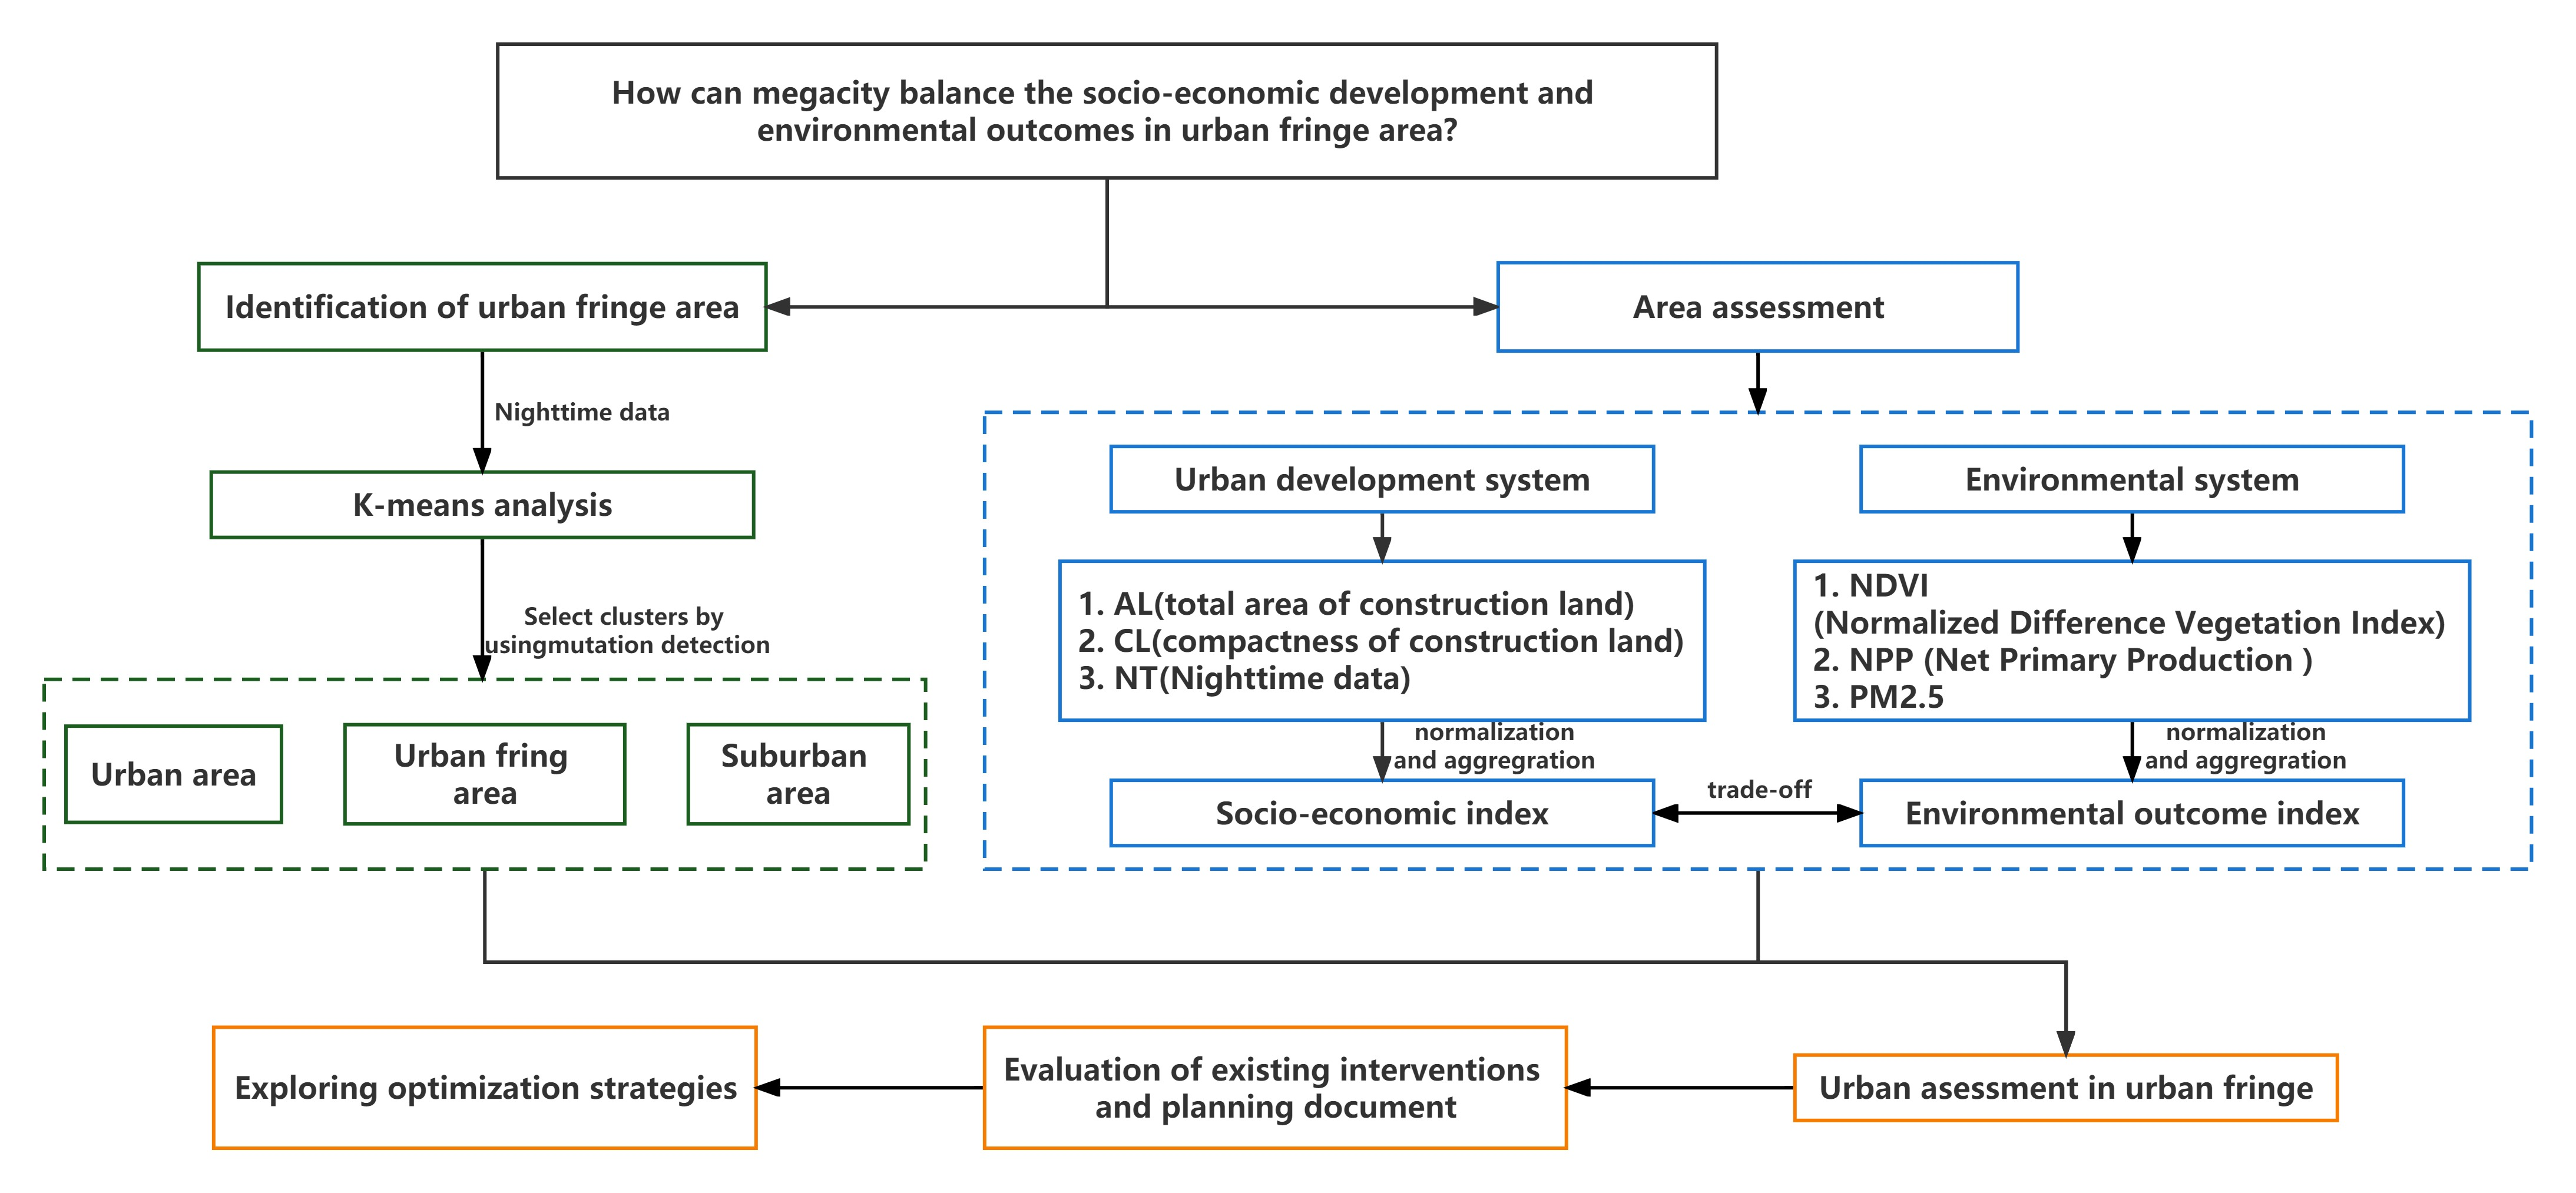
\includegraphics[width=15cm]{Figure/framework0821.jpg}
}
\caption{The framework of the whole study process}
\label{structure}
\end{figure}
%%%%%%%%%%%%%%%%%%%%%%%

\subsection{Ethical Considerations}
The direction of the study was to understand the changing trends and policy orientation of the two systems in urban fringe area through the study of urban development and environmental system. In the context of climate change and urban sprawl, it would provide a sustainable development direction for urban fringe area in megacities.\\

Therefore, all data in this study were studied for the current geographical situation, economic and environmental situation of the area. All data could be publicly available through the Internet. And since the study was designed to analyze the data comprehensively from a larger perspective, the study wouldn't identify or reveal anything about the private lives and habits of individuals. In addition, the analysis results would be based on rigorous data analysis and provide reasonable conclusions and recommendations.\\


\subsection{Study area}

As the top cities in China for economic development, Guangzhou and Shanghai have relied on their coastal advantages to develop their urbanization in the last 30 years. While acting as the core of the metropolitan area, Guangzhou and Shanghai have been under great pressure on ecological space due to their rapid urbanization. Therefore, these cities would be used as case study cities in the study since both of them have similar economic status, geographic location and environment.\\

\subsubsection{Guangzhou}
As the central city in the Guangdong-Hong Kong-Macao Greater Bay Area, Guangzhou (Figure \ref{lulc}a) has a total area of 7434.4 km2. There would be a topographical structure of densely forested mountains in the northern area, which would act as the ecological support area of the whole city. Having the topography of hilly and basins, the central area of Guangzhou would be the socio-economic center. What’s more, with most proportion area of farmland, the southern area is now facing the situation of the urbanization process. Due to its special characteristics as a coastal port near the South China Sea, construction land in the southern area has expanded rapidly and there has been a huge population growth in about 500,000 when it comes to the total area. Therefore, Guangzhou would be one of the cities with urban sprawl problems between socio-economic system and environmental system in the Greater Bay Area \parencite{li_research_2021}.\\

\subsubsection{Shanghai}
Located in Yangtze River estuary, Shanghai (Figure \ref{lulc}b) is the economic center of China, with a permanent population of 7.16 million The total area of Shanghai metropolitan area is 6340.5km2 and it is near the South China. Surrounded by the land use type of farmland and forest, the central area is mainly construction land and the landscape type could be relatively simple. Besides, national natural habitats in Shanghai could prove high ecological value in ecosystem services \parencite{bing_spatial_2021}.\\
%%%%%%%%%%%%%%%%%%%%%%%%%%%%%%%%%%%%
\begin{figure}[h]
\centering
\subfigure[Guangzhou]{
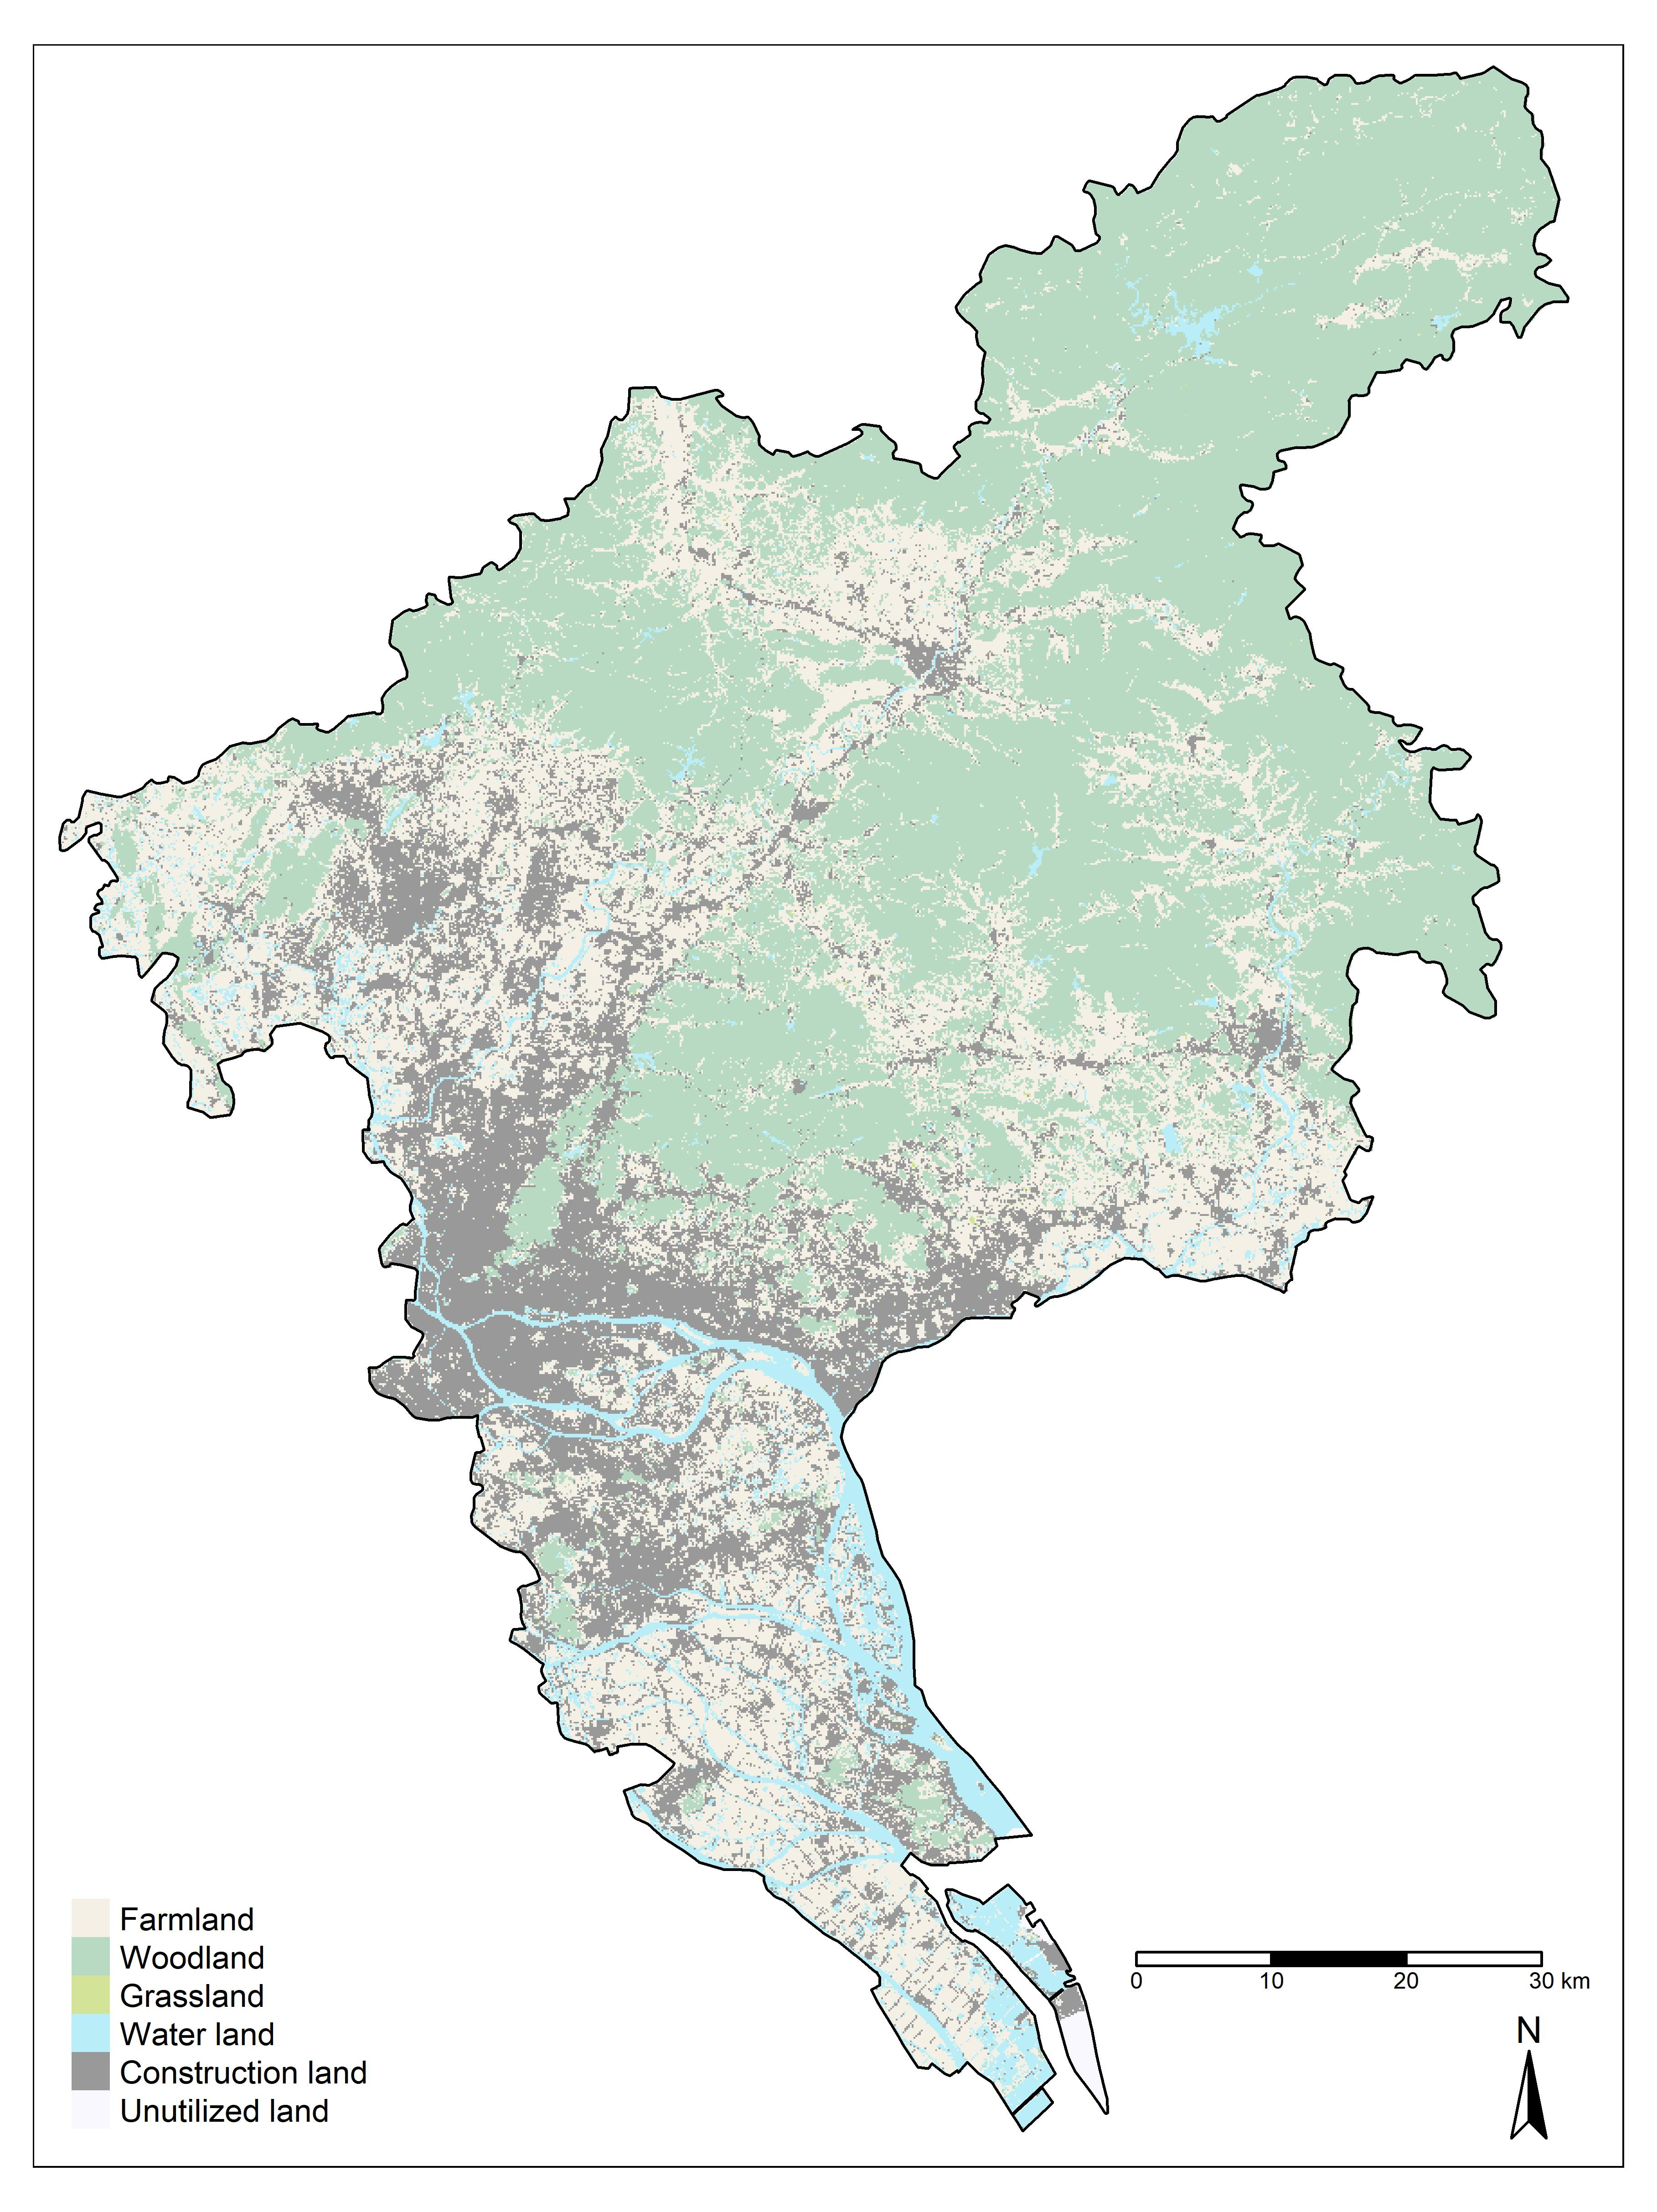
\includegraphics[width=6cm]{Figure/lulcgz.jpg}
}
\quad
\subfigure[Shanghai]{
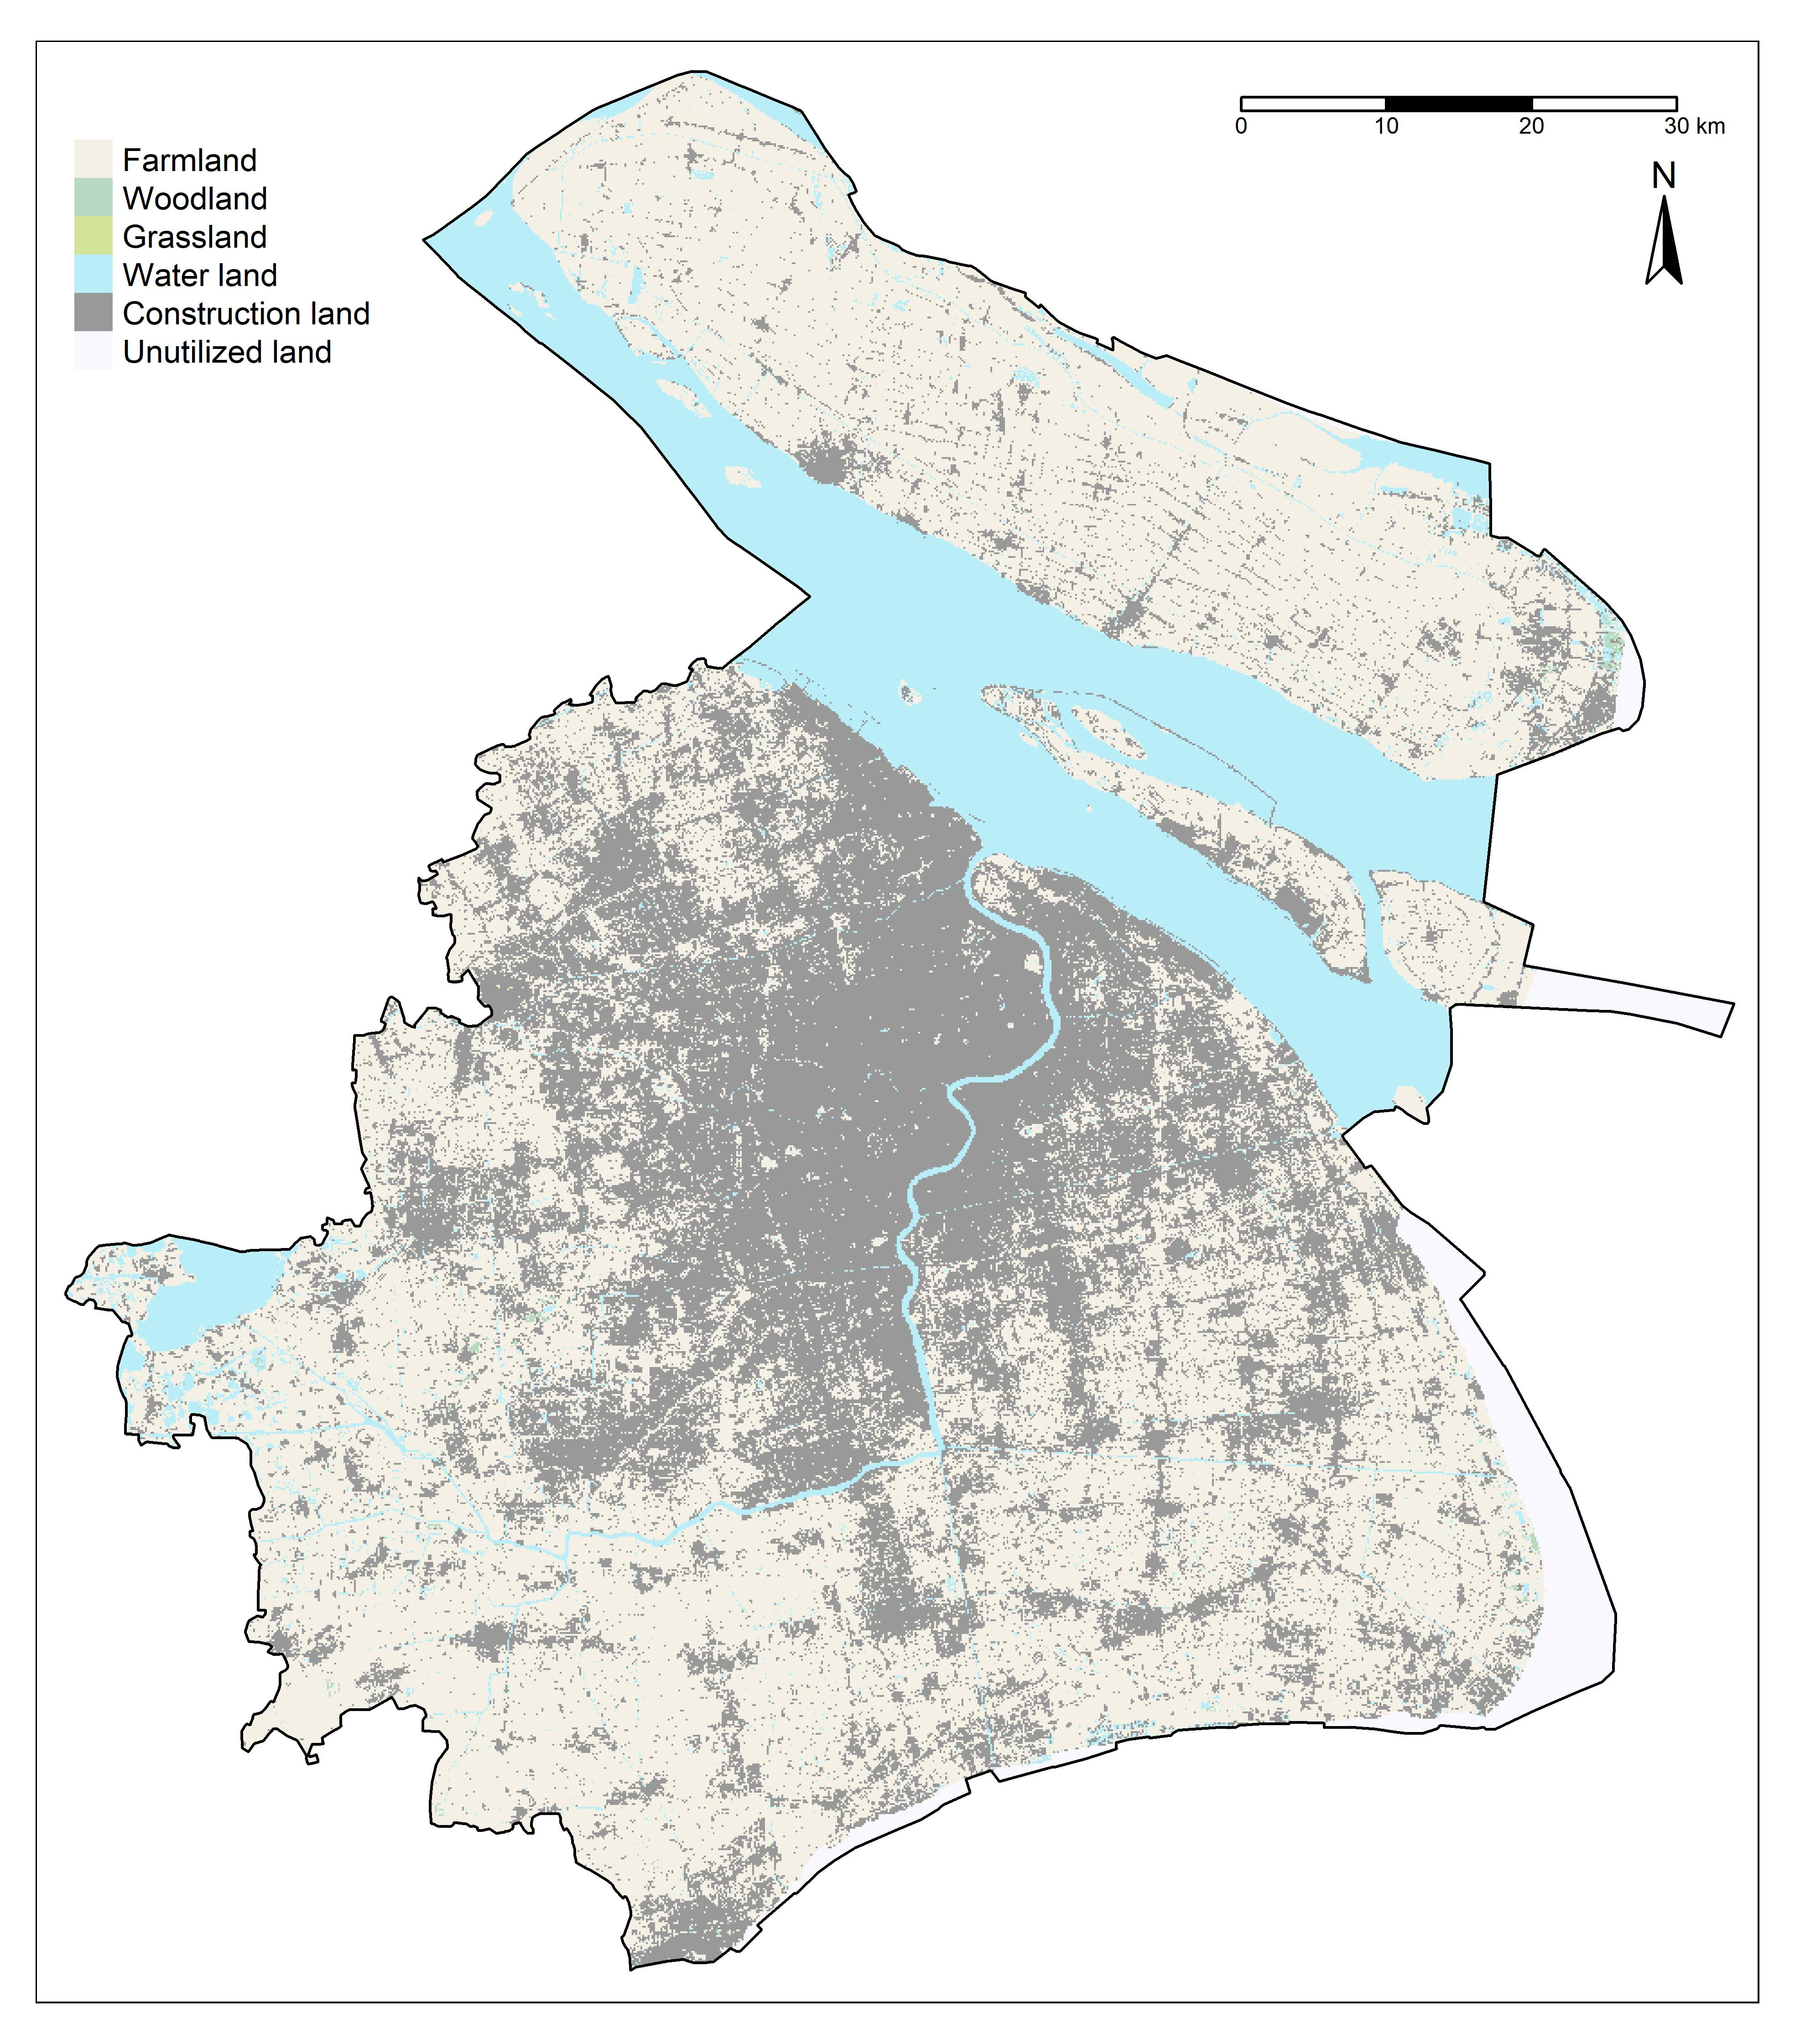
\includegraphics[width=7cm]{Figure/lulcsh.jpg}
}
\caption{Land use land cover of two case study cities}
\label{lulc}
\end{figure}
%%%%%%%%%%%%%%%%%%%%%%%%%%%%%%%%%%%%
\subsection{Dataset}
As this study requires data collection and analysis from the perspective of urban system and environmental system, the following data will be obtained and applied to the actual study.\\

\subsubsection{NDVI}
By using Landsat images on Google Earth Engine\href{https://github.com/Jackeytanlor/CASA_Dissertation/blob/main/code/GEE_NDVI}{(GEE)} remote sensing cloud computing platform, The 30m annual NDVI maximum dataset was used from 2013, 2016 and 2019. The NDVI data was calculated by using Landsat 8 remote sensing images from the US Landsat satellite. NDVI maximum for the research area was extracted from each month and generated the annual maximum data in each year. In Landsat 8, NDVI was calculated by using B5 and B4 bands.\\

\subsubsection{Net Primary Production (NPP)}
The global product MODIS (MOD17A3H V0006) Terra time series Net Primary Production (NPP)  at 500m spatial resolution and yearly compositing period was used from 2013, 2016 and 2019. The data source for this product is acquired through the United States Geological Survey (USGS) Land Process, and the data is merged and intercepted by \href{https://github.com/Jackeytanlor/CASA_Dissertation/blob/main/code/GEE_NDVI}{GEE} to produce data for the target area.\\

\subsubsection{PM2.5}
By using artificial intelligence and considering the spatio-temporal heterogeneity of air pollution, PM2.5 from The China High Air Pollutants \href{https://weijing-rs.github.io/product.html}{(CHAP)} dataset was used from 2013, 2016 and 2019. The data source for this product, ground-level air pollution in China, could have long-term, full-coverage, high-resolution and high quality \parencite{wei_chinahighpm10_2021}. The dataset is acquired through open access link, and the data is merged and intercepted by R to extract data for the target area.\\

\subsubsection{Land use land cover (LULC)}
By using Landsat images on GEE, Landsat-derived annual land cover product of China (CLCD) from 2013, 2016 and 2019. In order to improve the spatial-temporal consistency of LULC compared with Landsat dataset, the dataset used a post-processing method, which may include spatial-temporal filtering and logical reasoning \parencite{yang_30_2021}. The dataset is acquired through \href{https://doi.org/10.5281/zenodo.4417810}{Zenodo} (\url{https://doi.org/10.5281/zenodo.4417810}).\\

\subsubsection{Nighttime data (NT)}
The global Nighttime data Suomi-NPP VIIRS-derived nighttime lights at 500m spatial resolution and yearly compositing period was used from 2013, 2016 and 2019. The data source for this product is acquired through National Oceanic and Atmospheric Administration \href{https://github.com/Jackeytanlor/CASA_Dissertation/tree/main/dataset/NT}{(NOAA)}.\\

\subsection{Methods}
\subsubsection{Identification of urban fringe area}
\subsubsubsection{Fluctuation theory}
Due to production and lifestyle differences, citizens from urban area are more likely to use light at night and it would be much more than those who live in suburban area. From urban area to urban fringe and suburban area, nighttime lighting tensity would change to decrease followed by the gradual decrease of urbanization development level. On the other hand, the NT value within urban area and suburban area will be in a flat state because the land use type is relatively single and has not been affected in a short period of time. However, Due to the excessive impact of being in the city center to the countryside in urban fringe area, there might be more complex in land use type, which would show the characteristic of shows characteristics of transition, diversity, and fluctuation. The area will be influenced by urbanization in a short period of time, so the NT value in the area will be in a fluctuating state. Therefore, NT value will show a 'smooth-fluctuating-smooth' characteristic as the surrounding environment changes from urban area to urban fringe and suburban area. Based on the existing NT value change characteristics, a combined–value method was used to identify urban fringe area \parencite{yang_spatial_2017}.\\

According to the combined-value method, cluster analysis would be used in the identification of urban fringe area. When it comes to the selection of cluster analysis methods, the K-means analysis would be a popular method for identifying urban areas. Although the cluster method of K-means may have a shortage of low sensitivity to initial points because of its clear clustering structure and simple clustering process. The method would be not only easy to use but also avoids the errors from clustering methods such as DBSCN due to land use dispersion \parencite{feng_using_2020}.\\

By using a given number of clusters n and dataset containing different dimensions of data objects as input, K-means analysis can comprehensively compare the attributes and values of different data objects. Finally, the model would output object with the highest similarity in the same cluster.\\

\subsubsubsection{Nighttime light and Light Fluctuation}
According to the combined–value method, 2 dimensions of the data objects would be introduced in the K-means analysis. NT value would be one aspect of the data object, since it can show the light intensity, which can show the difference between central area and the non-central area. However, the accuracy of the data may not be as accurate as in a developed country, which may result in a small amount of error \parencite{zhang_can_2013}.\\

Light fluctuation would be the second data object. The degree of fluctuation of light intensity would help to explore the degree of variation of the light intensity in a certain range, which can do help to find the urban fringe area. Therefore, the study used two indicators, nighttime index and nighttime fluctuation, to perform a cluster analysis of the area, which allows for a more accurate identification of the area in two dimensions.\\

\subsubsubsection{Calculation of light fluctuation}
The calculation of the degree of fluctuation of light intensity(DF) would be shown as below:\\

\begin{equation}
DF=NT_{max}-NT_{min}
\end{equation}

Where DF is the degree of fluctuation. $NT_{max}$ and $NT_{min}$ would be the maximum and minimum value of nighttime light intensity.\\

According to the relevant research, in order to calculate the DF value, $NT_{max}$ and $NT_{min}$ should be selected in the 3*3 neighborhood by using neighborhood analysis \parencite{feng_using_2020}. It can find the exact fluctuation value from the smallest range of raster data.\\

In order to process K-means analysis with these two objects, normalization of the data would be required. Max-Min normalization should be used to standardize the data from 0 to 1. The calculation of normalization would be shown as below:\\

\begin{equation}
NT_{nor}=\frac{NT-NT_{min}}{NT_{max}-NT_{min}}
\end{equation}
\begin{equation}
DF_{nor}=\frac{DF-DF_{min}}{DF_{max}-DF_{min}}
\end{equation}

Where $NT_{nor}$ is the normalization value of nighttime light intensity; $DF_{nor}$ is the normalization value of the degree of fluctuation.\\

\subsubsubsection{Selection of clusters}
Since the K-means analysis in this study needs to explore the clusters of n in the two study area and find the value of n that best matches the study area. Since the research would need to find out 3 kinds of area: urban area, urban fringe area and suburban area, n should be started with 3. Besides, by adjusting the parameter of n, the study can find that the space in the different clusters becomes fragmented as the value of n increases. As the number of clusters rises, so does the complexity of the area \parencite{yang_spatial_2017}. When n \textgreater 10, clusters will intersperse in space, which is not conducive to the application of this study from the study area to other areas. Therefore, a total of 3-10 clusters are presented by the k-means method and the most suitable clusters would be selected by combining the performance of the two urban indicators in the urban fringe area. \\

In the meanwhile, according to research, in order to find the most suitable clusters in case study cities, it is necessary to use mutation detection to observe the result of cluster analysis and compare it with 2 objects. In this study, a straight line is drawn in 2 objects and the line will pass through as many clusters as possible. through this line, a section of the map would be shown and the variation and fluctuation of 2 objects in this section will be shown in the graph (Figure \ref{cluster7}). By comparing the fluctuations of Land use, NT and DF values, the study will select the most suitable n value as the best cluster number.\\

By comparing fringe area identified from the planning document from Guangzhou and Shanghai, 7 clusters are more able to show the mutation values in the area. According to Figure \ref{section}, it could be found that when the section line in Figure \ref{section}ab moves from south to north, the NT and DN values showed fluctuations with the position. It is obvious that some areas showed a significant decrease in DN value when NT value was at the highest point, which could be considered in Cluster n=7(Figure \ref{section}bc) This could demonstrate that the clustering of edge regions could be more clearly identified when there were multiple clusters. Therefore, 7 clusters were used as the final cluster for identification in this study. Therefore, the study may choose n=7 as the result and merge different cluster into 3 area, urban area, urban fringe area and suburban area.\\

%%%%%%%%%%%%%%%%%%%%%%%%%%%%%%%%%%%%
\begin{figure}[h]
\centering
\subfigure[Guangzhou]{
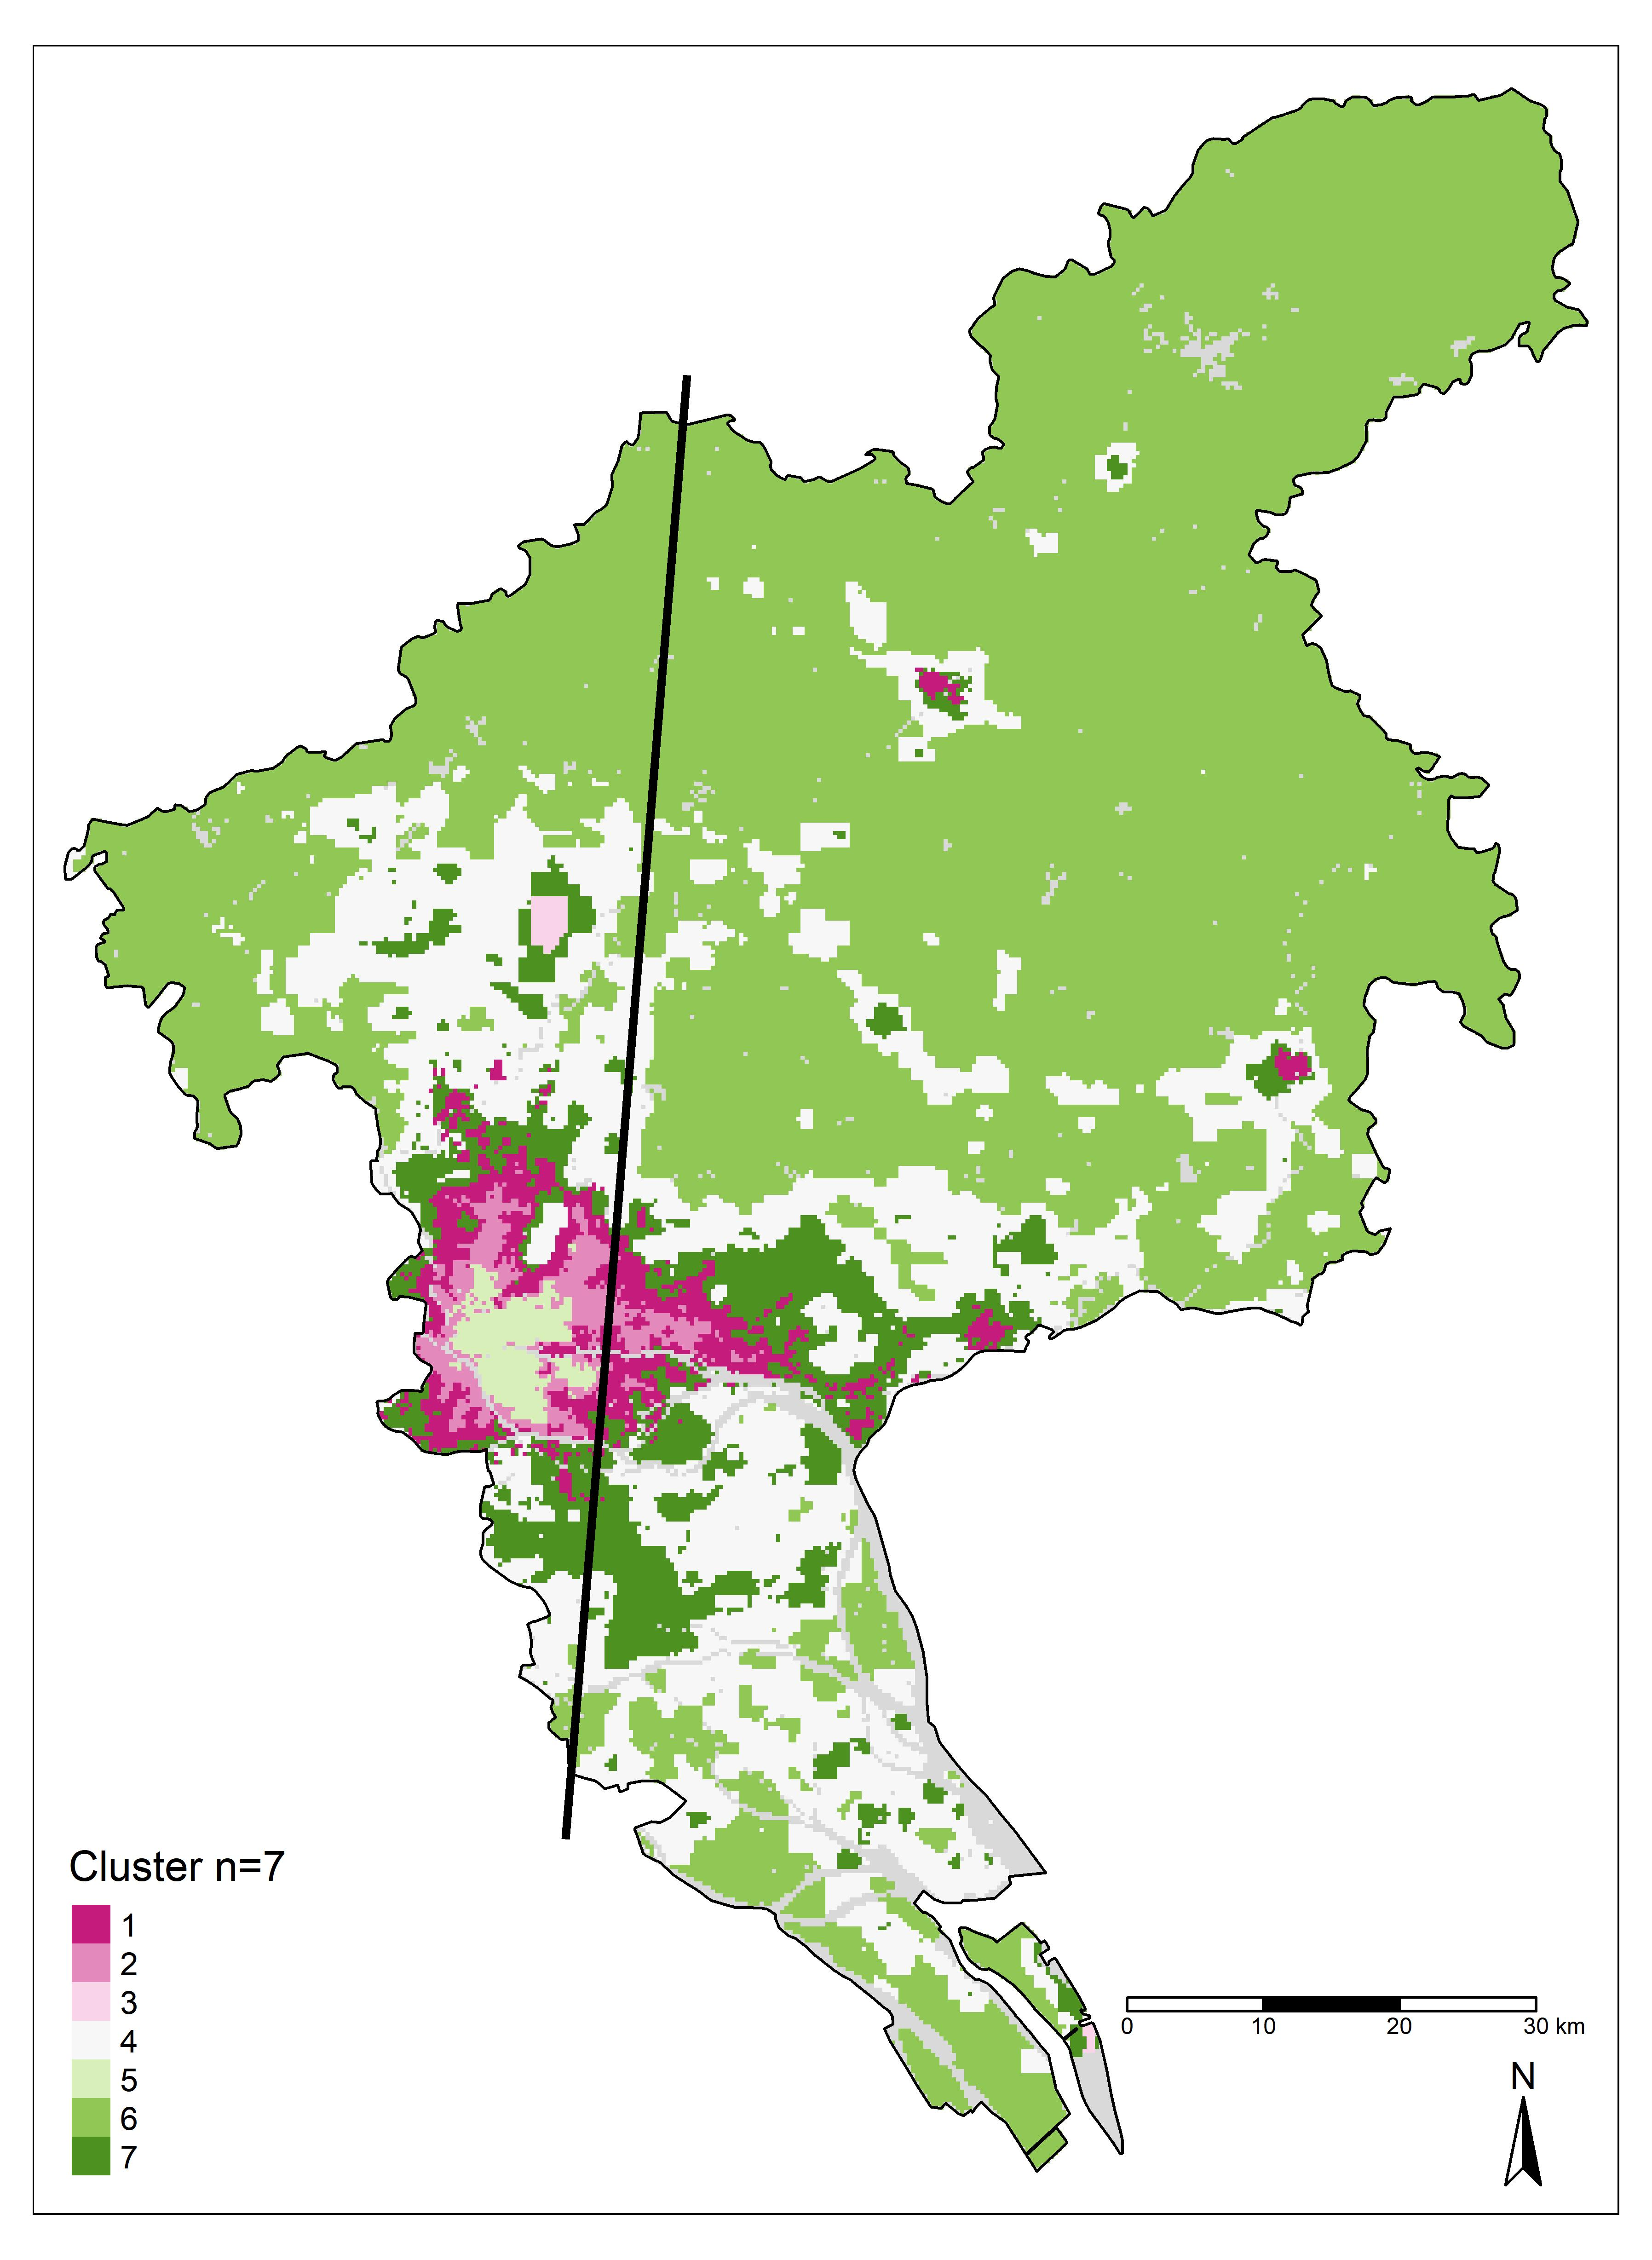
\includegraphics[width=6cm]{Figure/cluster7_0821.jpg}
}
\quad
\subfigure[Shanghai]{
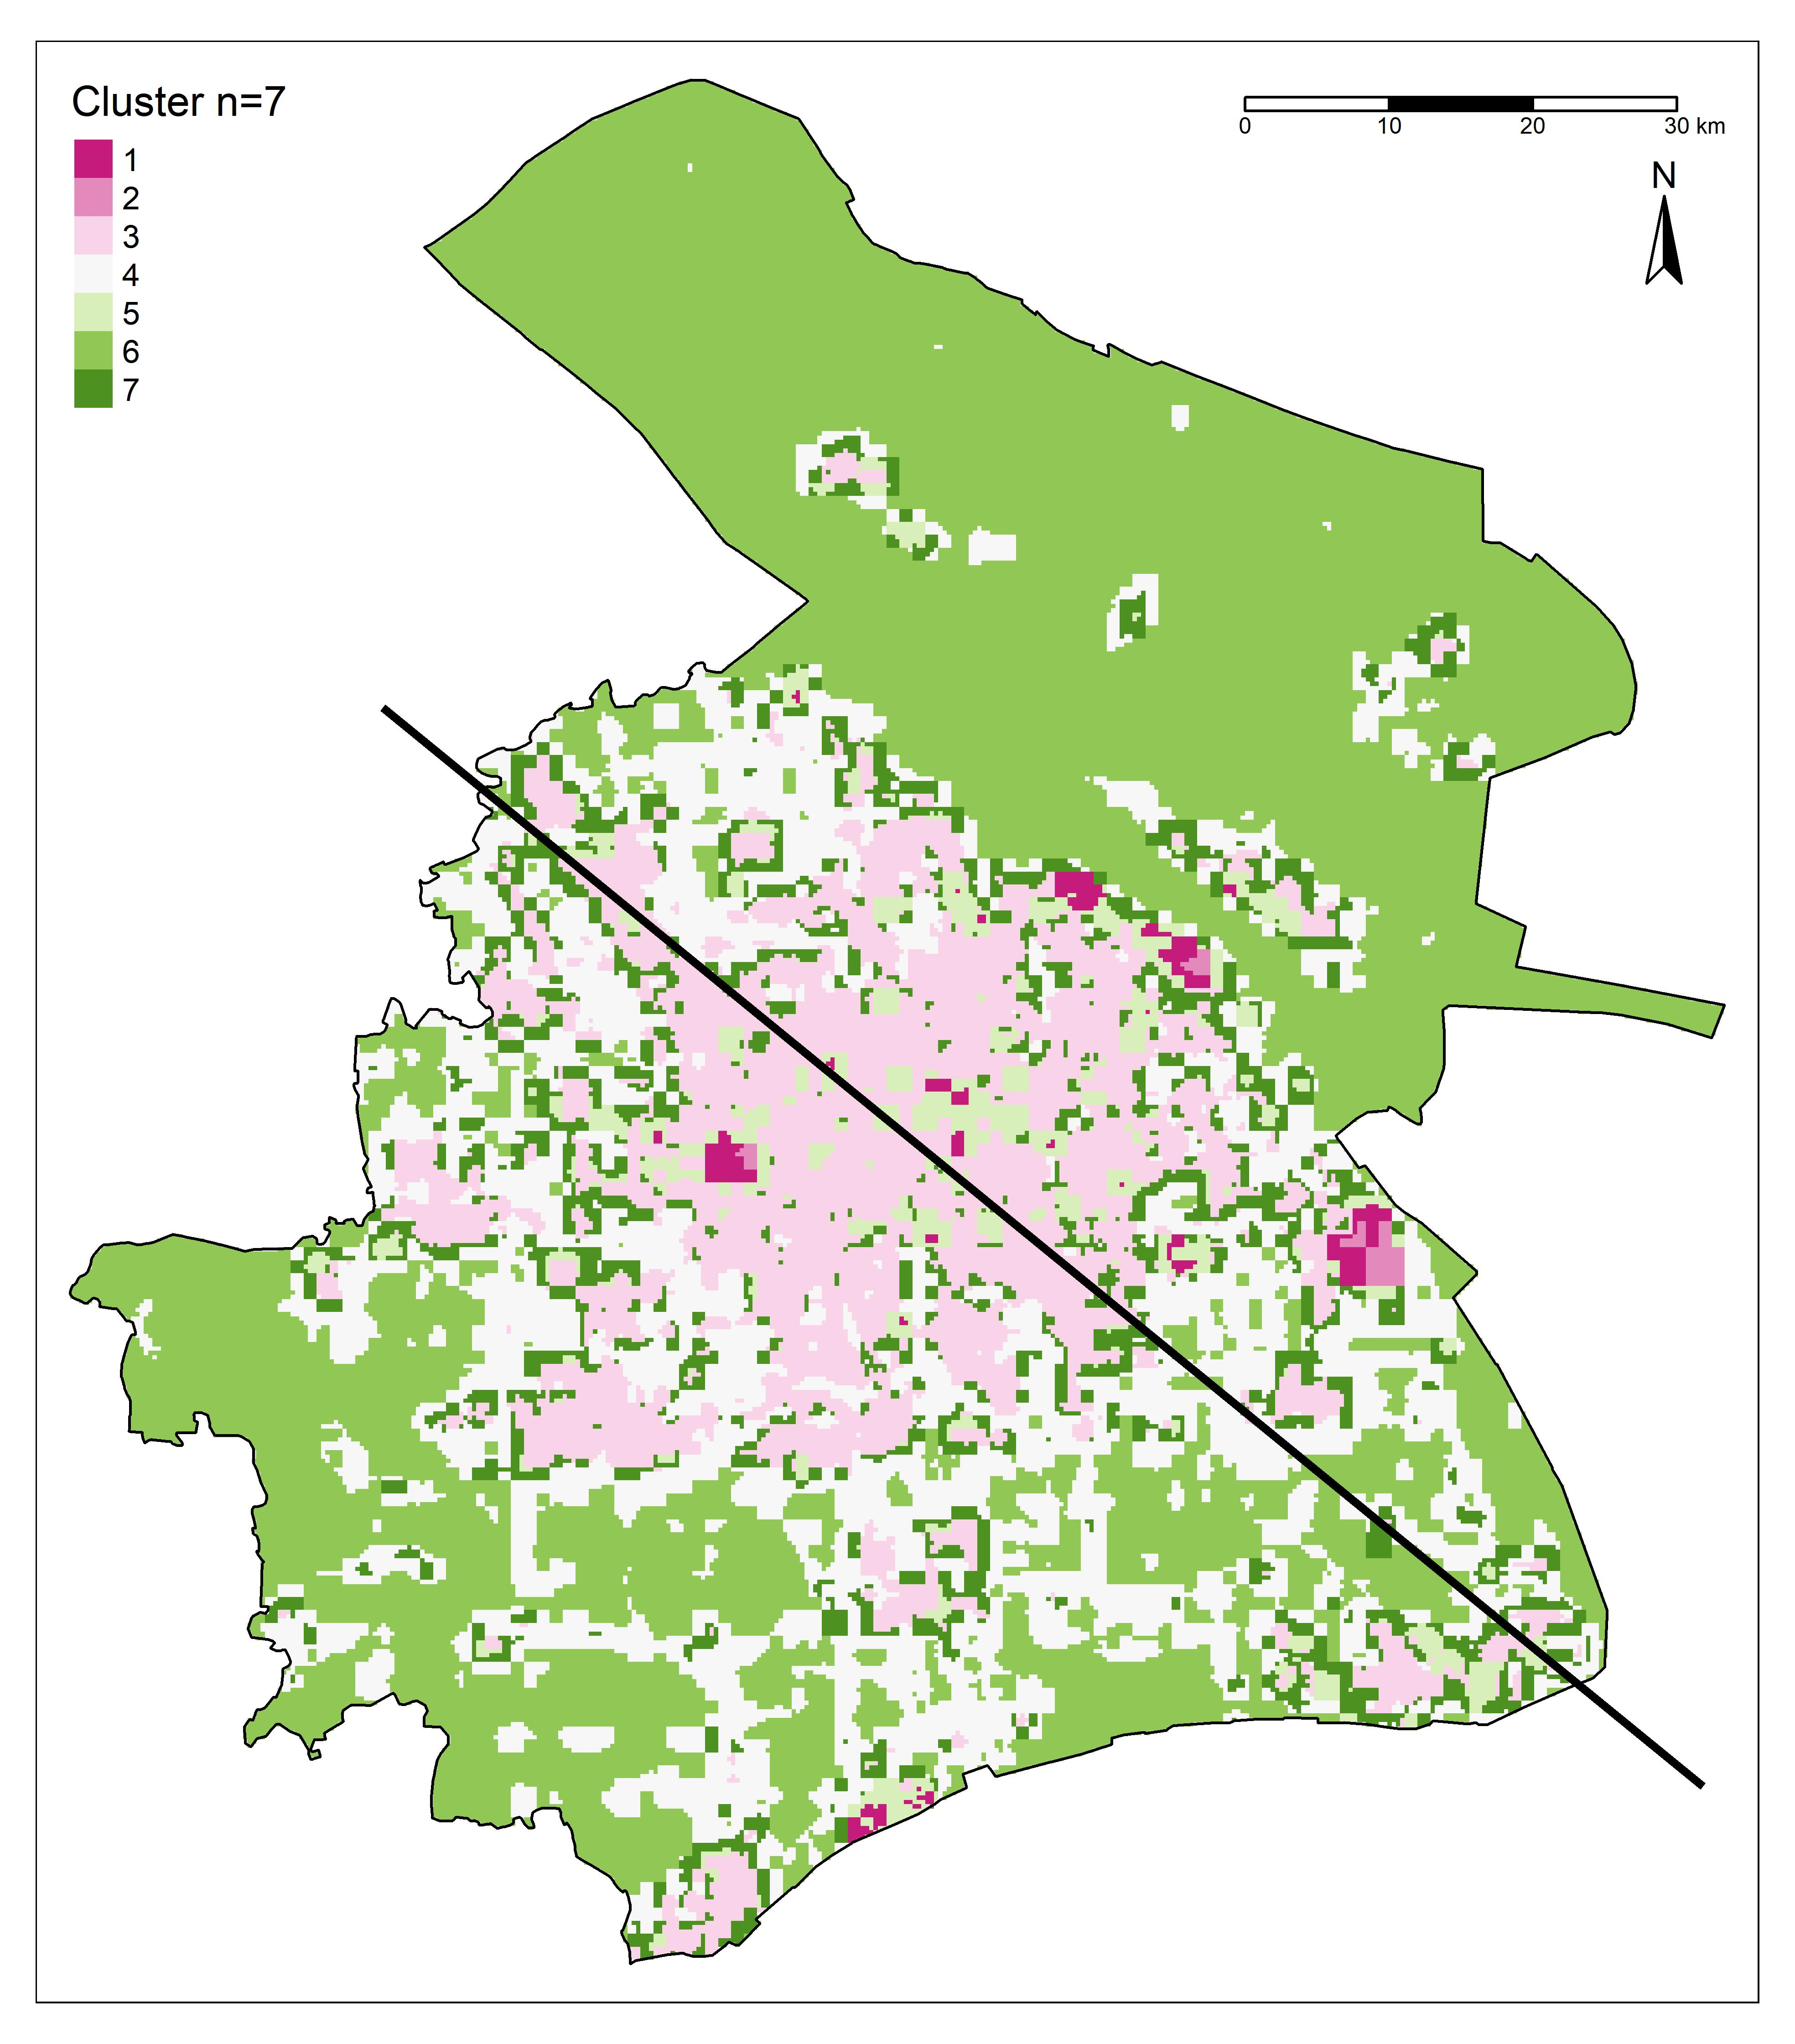
\includegraphics[width=7cm]{Figure/clustersh7_0821.jpg}
}

\caption{The distribution result of clusters (n=7) in the study area with section line}
\label{cluster7}
\end{figure}
%%%%%%%%%%%%%%%%%%%%%%%%%%%%%%%%%%%%

%%%%%%%%%%%%%%%%%%%%%%%%%%%%%%%%%%%%
\begin{figure}[h]
\centering
\subfigure[Guangzhou]{
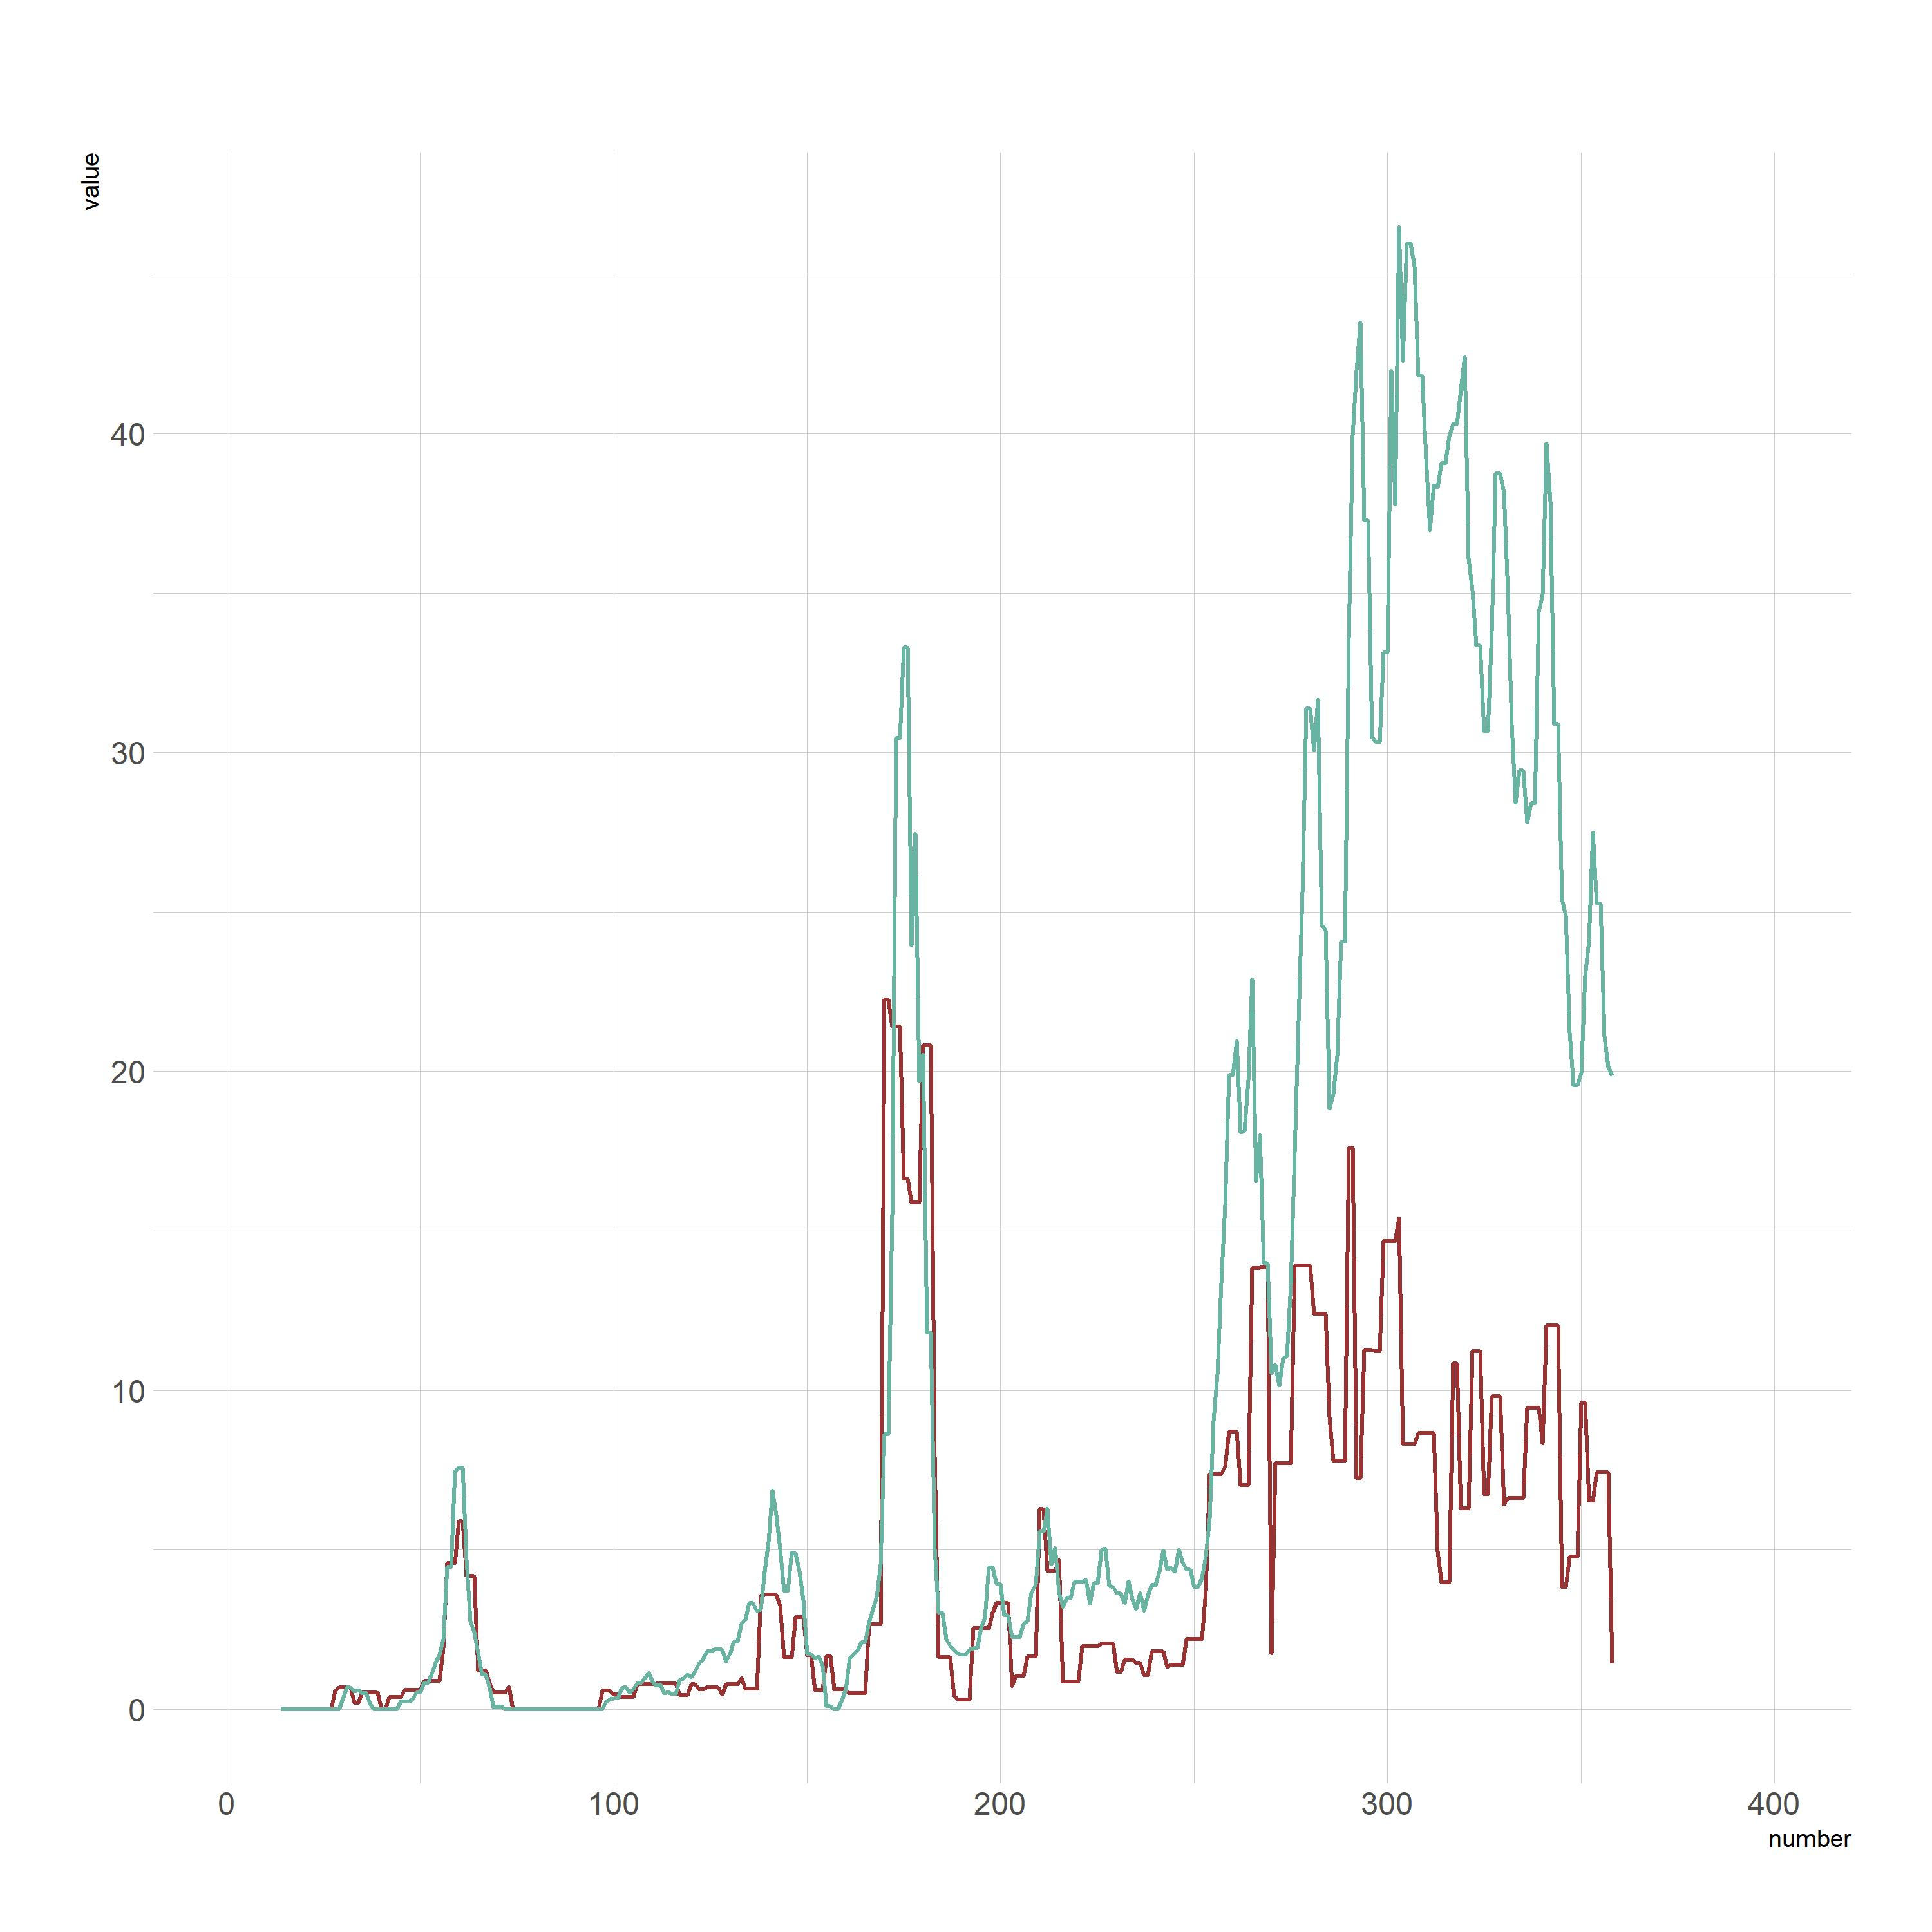
\includegraphics[width=6cm]{Figure/nt0821.jpg}
}
\quad
\subfigure[Shanghai]{
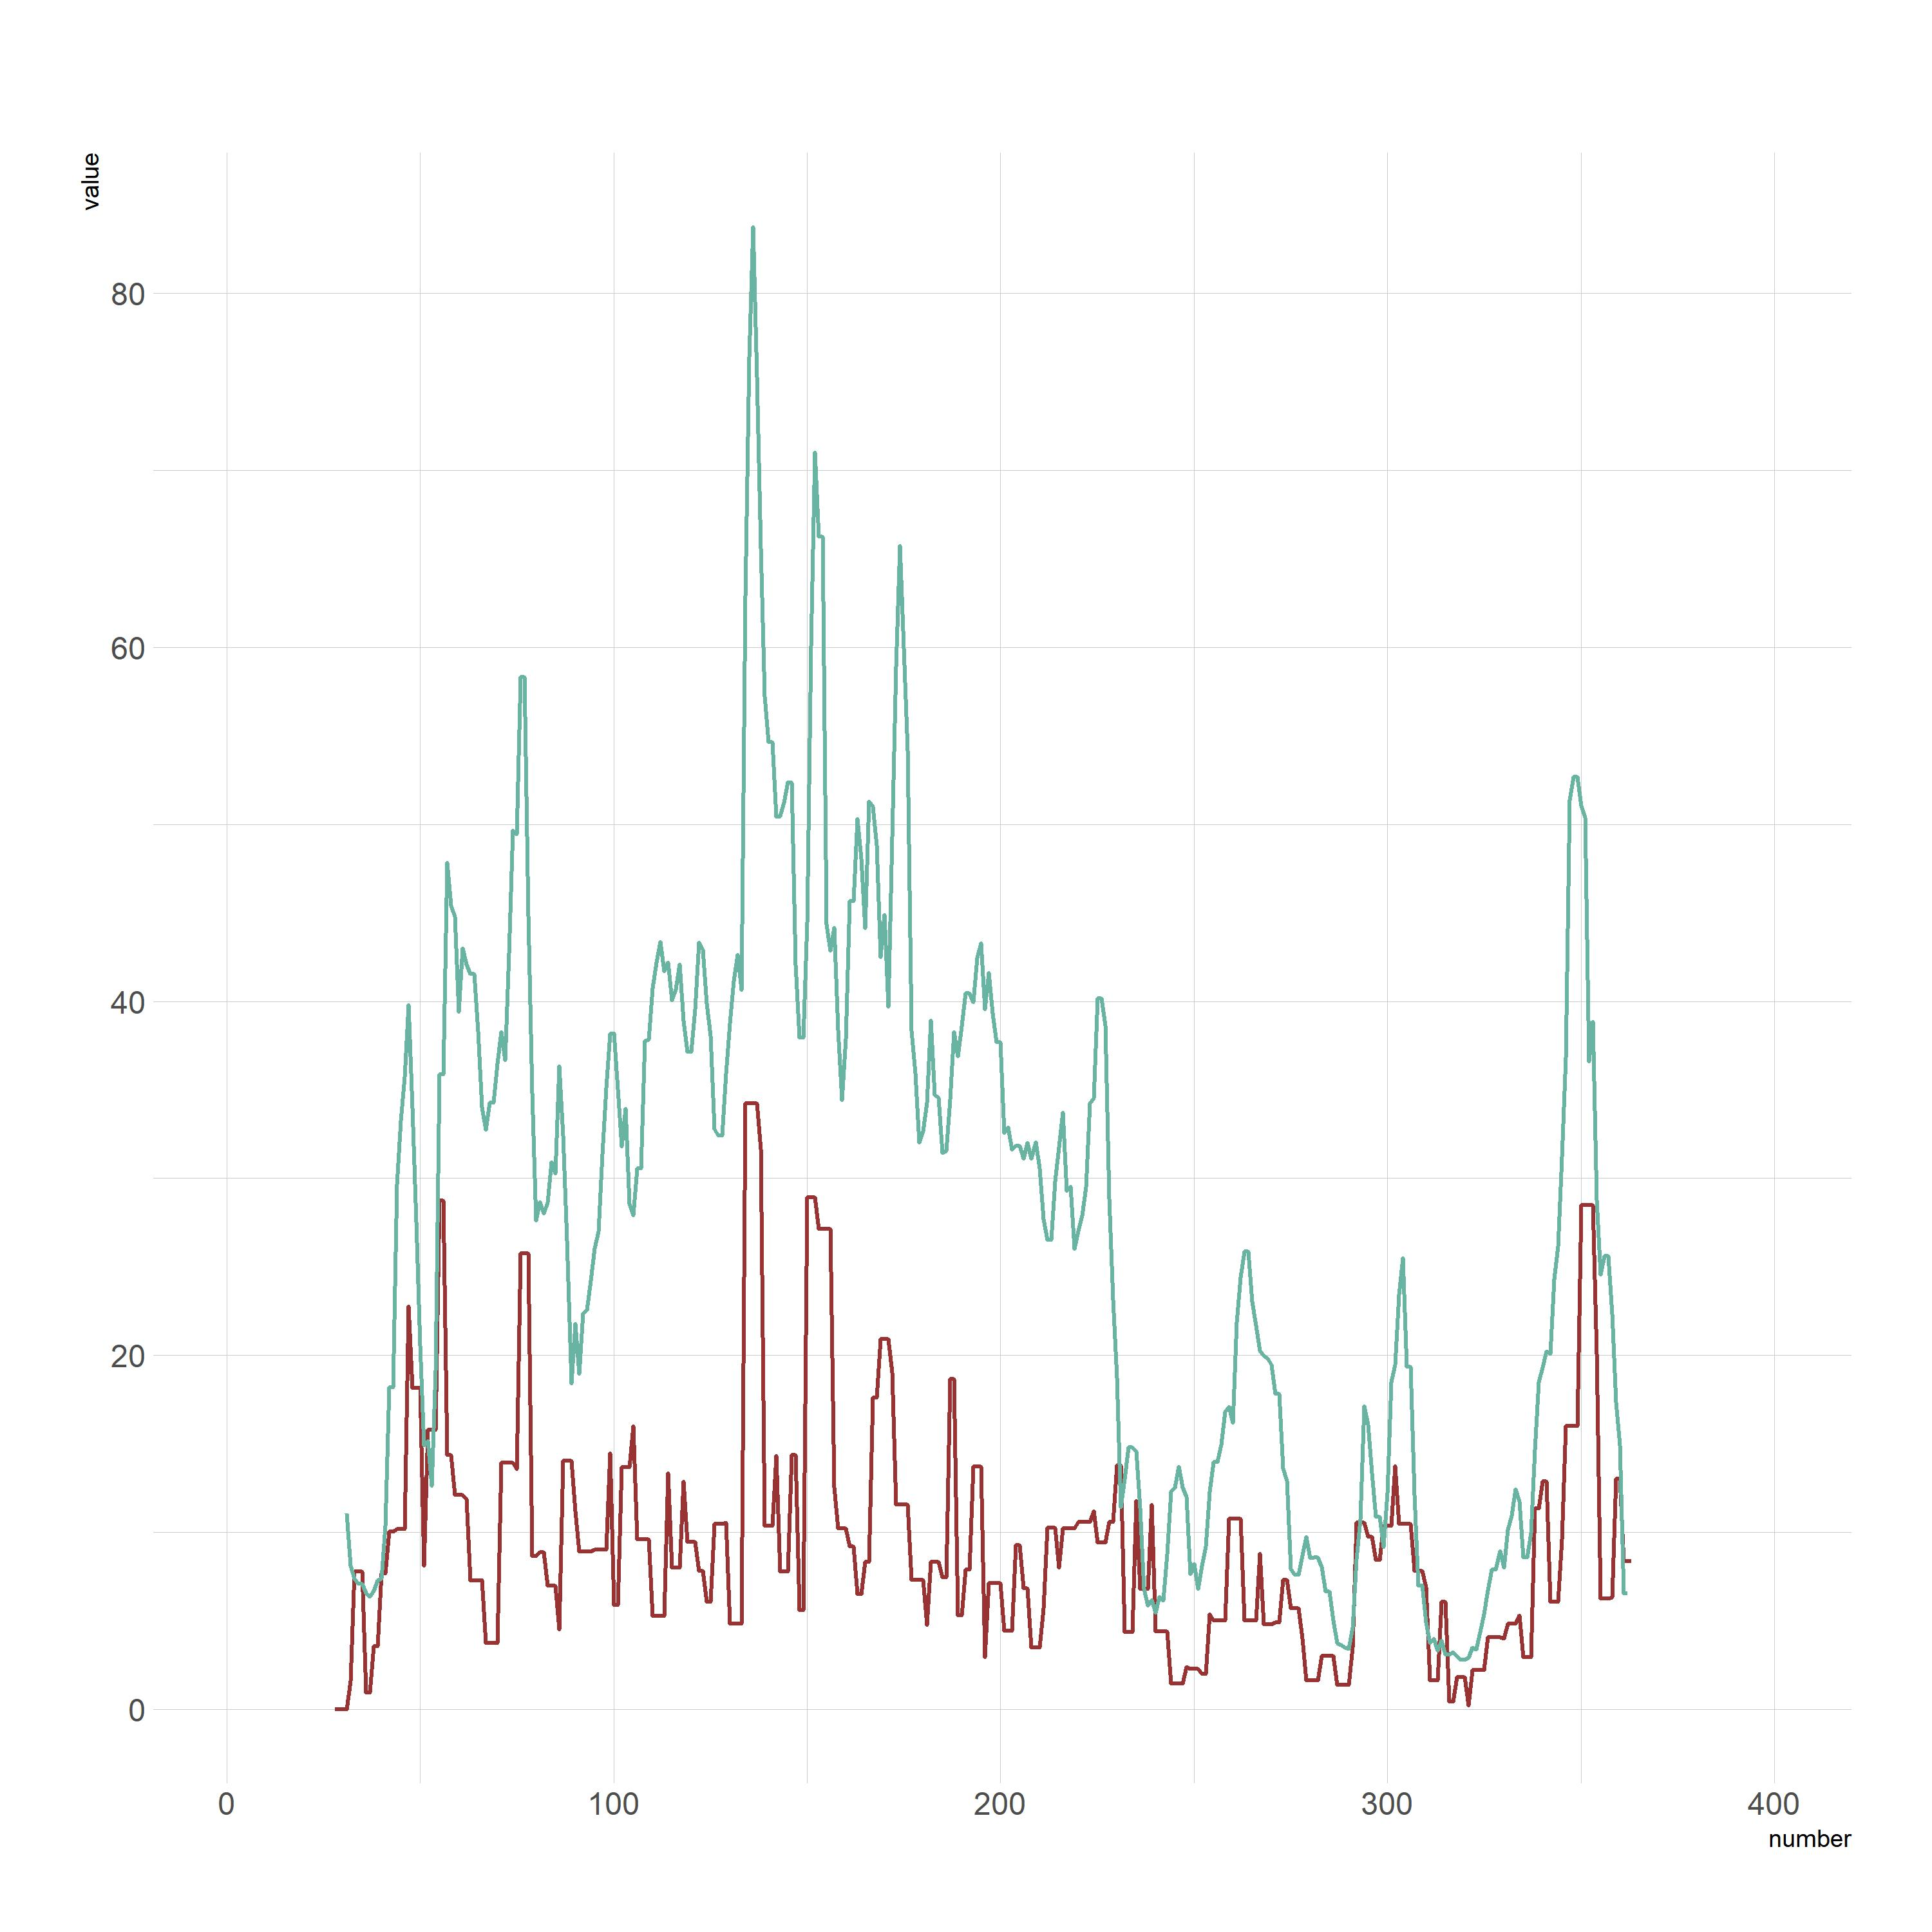
\includegraphics[width=6cm]{Figure/nt_sh0821.jpg}
}
\quad
\subfigure[Performance of section line in cluster n=7(Guangzhou) ]{
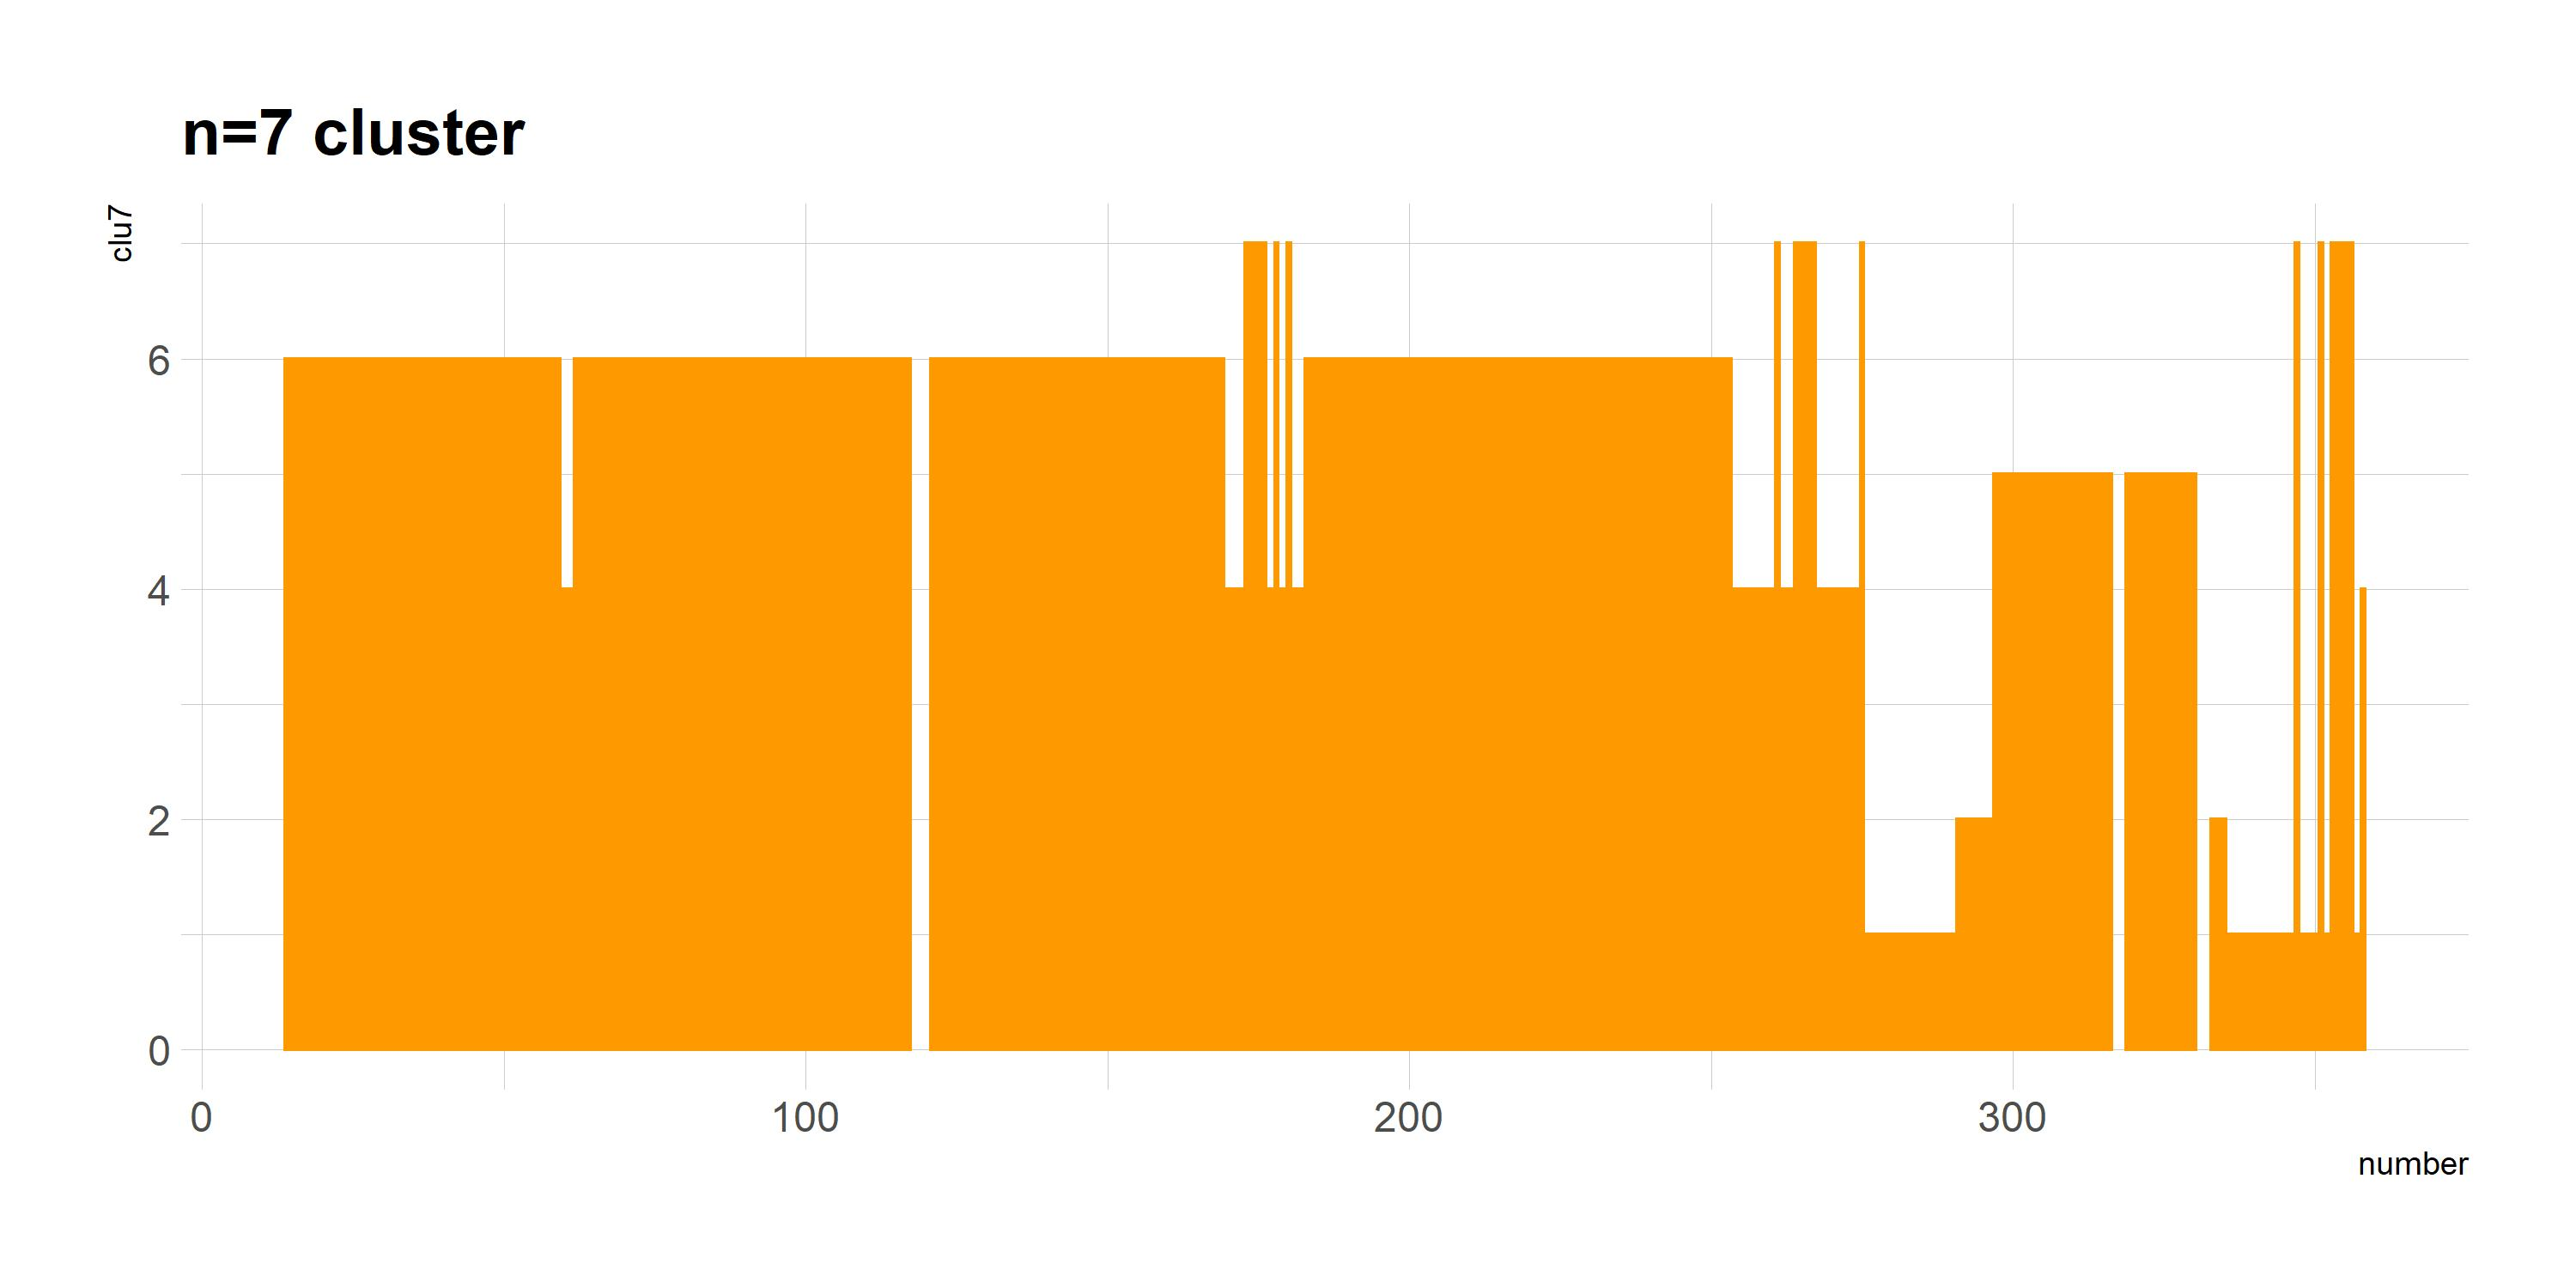
\includegraphics[width=6cm]{Figure/n7.jpg}
}
\quad
\subfigure[Performance of section line in cluster n=7(Shanghai) ]{
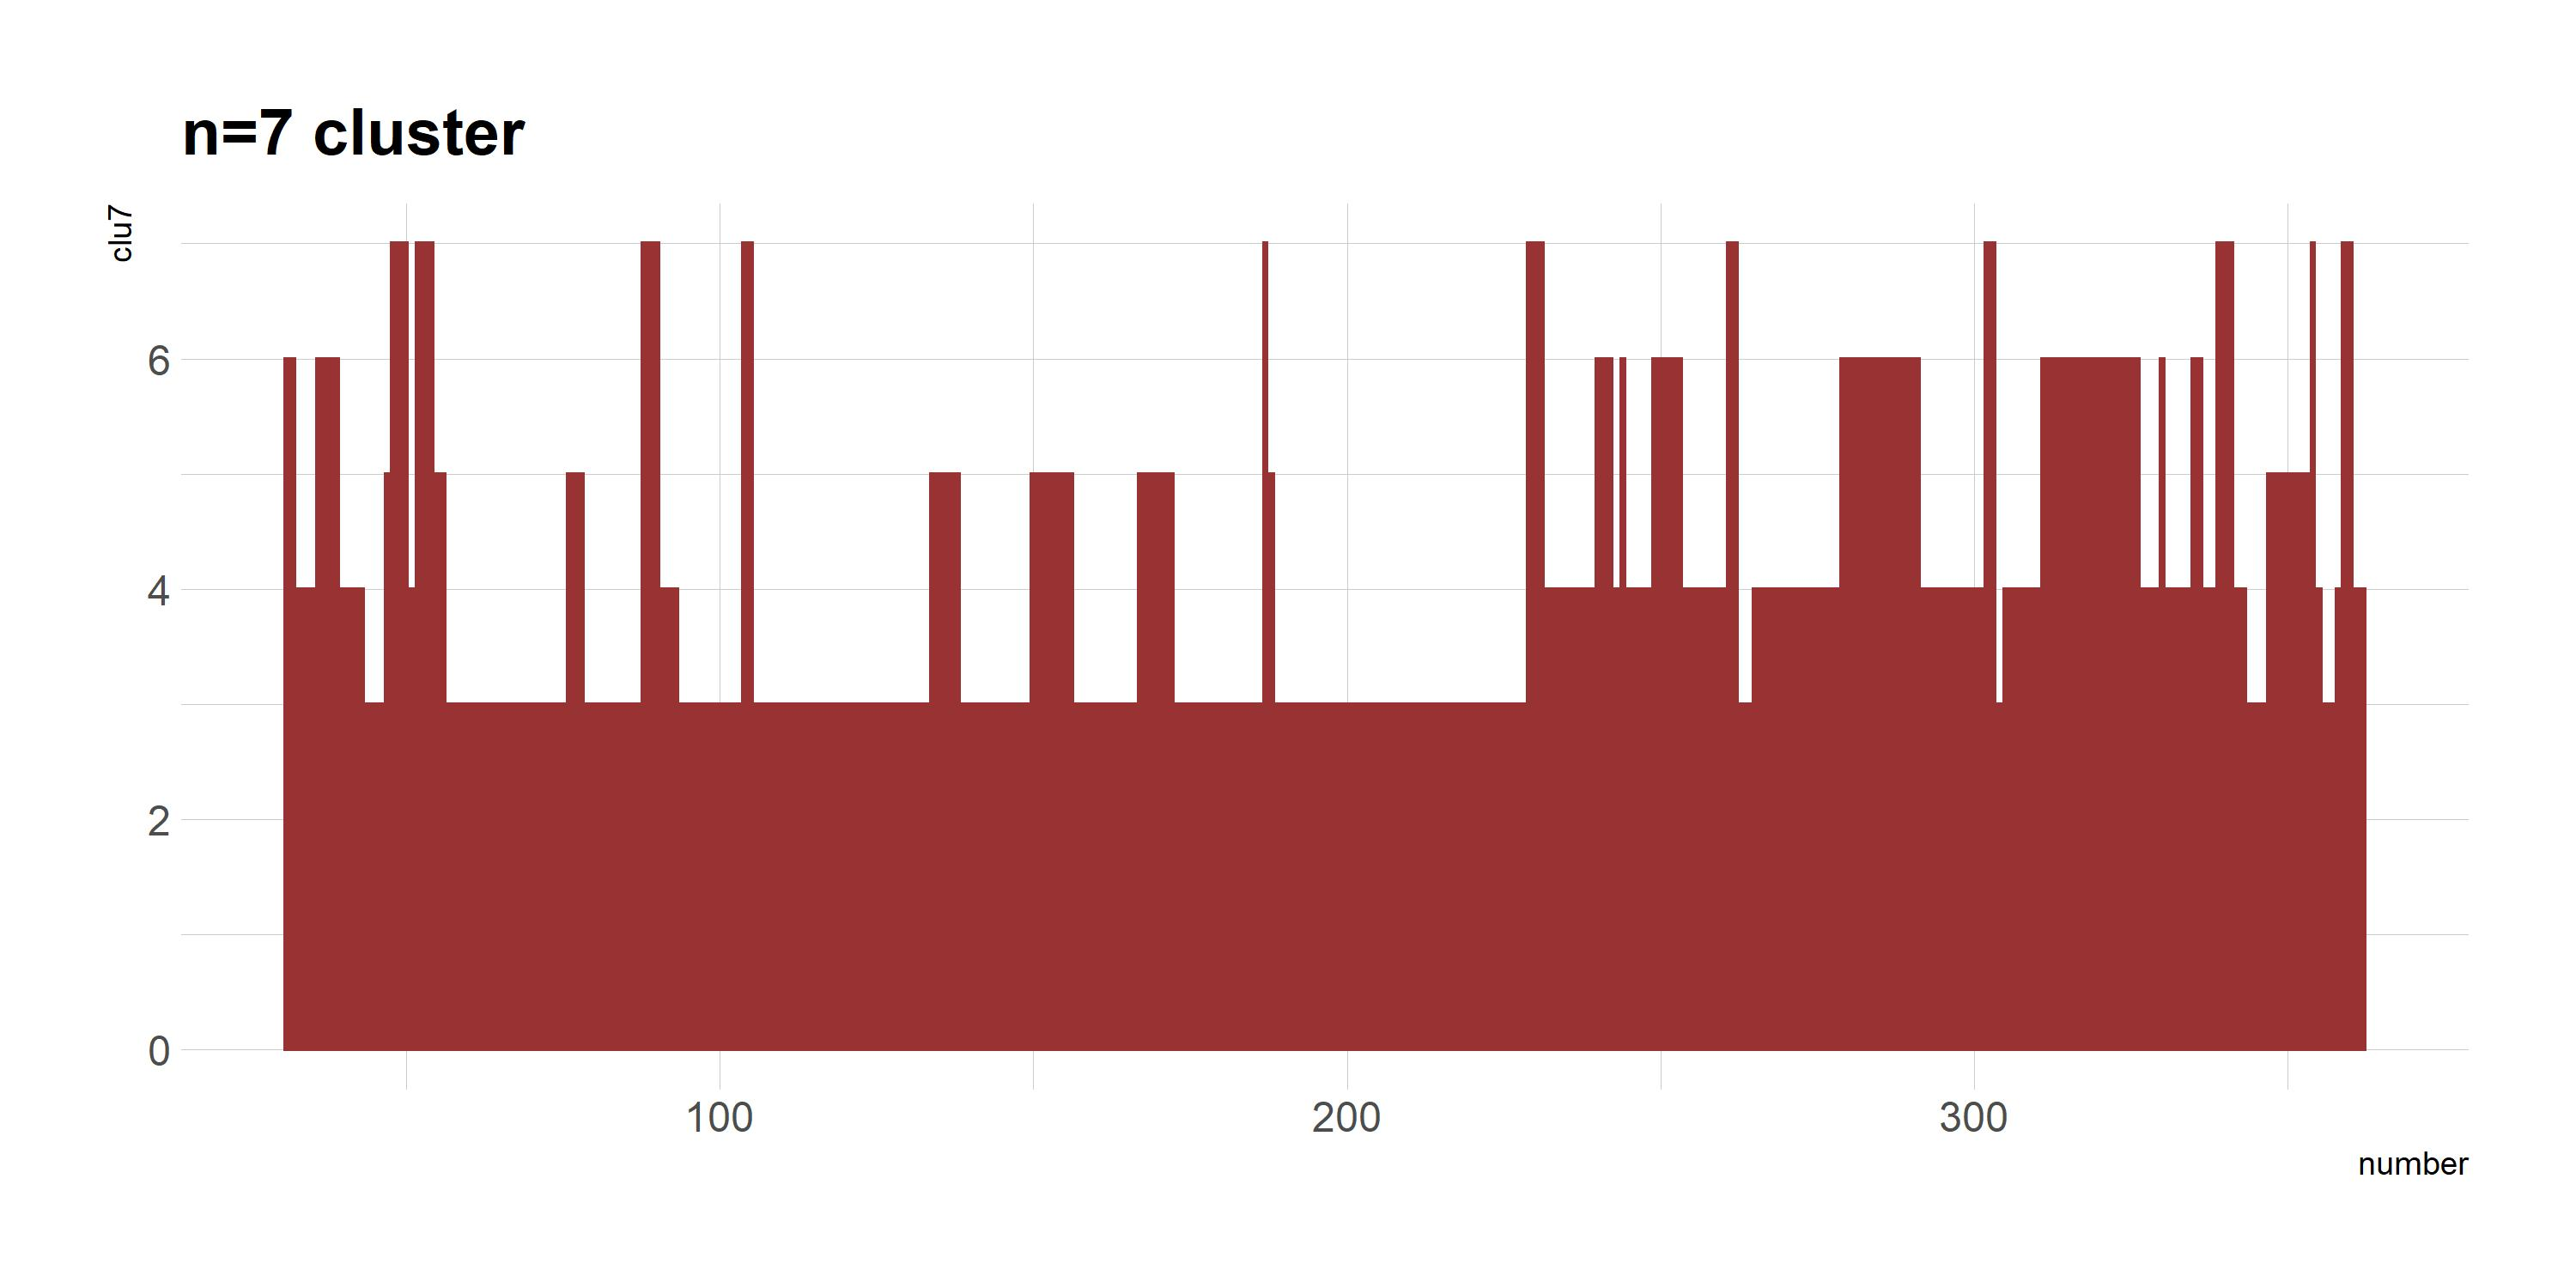
\includegraphics[width=6cm]{Figure/n7_sh.jpg}
}
\caption{The fluctuation of NT and DF values with section lines moving from south to north when n=7}
\label{section}
\end{figure}
%%%%%%%%%%%%%%%%%%%%%%%%%%%%%%%%%%%%

\subsubsection{Evaluation of socio-economic and environmental system}
As shown in Table \ref{description}, in order to evaluate the socio-economic and environmental system, 6 indicators from 2 systems were selected to assess the urban development and environmental outcomes.
%%%%%%%%%%%%%%%%%%%%%%%%%%%%%%%%%%%%%%%%%%%%%%%%%%%%%%%
\begin{table}[H]
\caption{The description of indicators in area evaluation}
\label{description}
\centering
\begin{tabular}{>{\hspace{0pt}}m{0.148\linewidth}>{\hspace{0pt}}m{0.6\linewidth}>{\centering\arraybackslash\hspace{0pt}}m{0.165\linewidth}} 
\hline
\multicolumn{1}{>{\centering\hspace{0pt}}m{0.148\linewidth}}{\textbf{Indcator}} & \multicolumn{1}{>{\centering\hspace{0pt}}m{0.6\linewidth}}{\textbf{Description}} & \textbf{Unit}  \\ 
\hline
\textbf{AL}                                                                     & Total area of construction land                                                    & \%             \\
\textbf{CL}                                                                     & Compactness of construction land                                                   & \%             \\
\textbf{NT}                                                                     & Nighttime data                                                                     &                \\
\textbf{NDVI}                                                                   & Normalized Difference Vegetation Index                                             &                \\
\textbf{NPP}                                                                    & Net Primary Production                                                             & $gc/(m^{2}*a)$      \\
\textbf{PM2.5}                                                                  & Air pollutants                                                                     & $\mu g/m^{3}$          \\
\hline
\end{tabular}
\end{table}
%%%%%%%%%%%%%%%%%%%%%%%%%%%%%%%%%%%%%%%%%%%%%%%%%%%%%%%
\subsubsubsection{Socio-economic system}
In order to evaluate the urban development of each case study city 3 dimensions of socio-economic indicators should be used to assess from the point of land development intensity. 
The first dimension is AL, which would refer to the total area of construction land in the grid of $300m \times 300m$ in this study. It could also be expressed as the area proportion of construction land in the assessing unit.\\
\begin{equation}
AL=\frac{A}{T}
\end{equation}
Where A is the total area of construction land; T is the assessing area.\\

The second dimension would be CL, which may refer to the compactness of construction land. According to research, it could define as the ratio of the area to the perimeter \parencite{peng_integrating_2020}. The calculation of CL would be chosen because of its high applicability and simple calculation process.\\
\begin{equation}
CL=\frac{A}{C}
\end{equation}
Where C is the length of individual construction land in the assessing unit.\\

The third dimension would be Nighttime light data. Since socio-economic activity could be positively correlated with the nighttime light data, NT could be also used to evaluate the socio-economic system. Compared with other indicators, since there has been a huge distance between the maximum value of NT and the medium value of NT, the study would take logarithms of the lighting data($NT_{log}$) as the assessment indicator.\\

What‘s more, with the resolution of $300m \times 300m$ in NT, in order to calculate the CL and AL value, the study would statistics in $300m \times 300m$ to ensure the standard of socio-economic data.\\

\subsubsubsection{Environmental system}
When it comes to the topic of climate change and air quality, 3 dimensions of indicators should be used to represent environmental outcomes.\\

The first dimension is NDVI, which can be referred to biodiversity from ecosystem service. The second dimension is NPP, with carbon fixation perspective. The last dimension is PM2.5, which have a different aspect of air pollution.\\

\subsubsubsection{Normalization of evaluation value}
In order to compare the socio-economic system and the environmental system from a comprehensive perspective, the indicators of each system would be integrated by means of normalization. The integration method would be shown as below:\\

\begin{equation}
IN_{i j norm}= \begin{cases}\frac{IN_{i j}}{\max IN_{i j}} & IN_{i j} \text { shows the larger the better } \\ \frac{\min IN_{i j}}{IN_{i j}} & IN_{i j} \text { shows the smaller the better } \\ \frac{\min \left(IN_{i j}, IN_{j}^{0}\right)}{\max \left(IN_{i j}, IN_{j}^{0}\right)} & \mathrm{IN}_{j}^{0} \text { is the ideal value with respect to } IN\end{cases}\\
\end{equation}
\begin{equation}
S_{i}=\frac{1}{n} \sum_{j=1}^{n} IN_{i j norm}
\end{equation}
Where $IN_{i j}$ is the value of each indicator, $S_{i}$ is the value of the normalization index.\\

When exploring each indicator, it was found that all the data except PM2.5 showed the larger the better trend. On the contrary, indicator PM2.5 showed the trend of the smaller the better. When using the formula to integrate each indicator, the study would generate socio-economic index and environmental index ranging from 0 to 1\\
